\documentclass{emulateapj}
\submitted{{\it Submitted for publication in ApJ}}
\usepackage{multirow,color,wrapfig,ulem}
\usepackage {graphicx}

\usepackage{graphics}
\usepackage[dvips]{epsfig}

\newcommand{\avg}[1]{\langle{#1}\rangle}  
\newcommand{\nscatt}{\langle N_{\rm  scatt}\rangle}
\newcommand{\ly}{{\ifmmode{{\rm Ly}\alpha~}\else{Ly$\alpha$~}\fi}}
\newcommand{\hMpc}{{\ifmmode{h^{-1}{\rm Mpc}}\else{$h^{-1}$Mpc }\fi}}   
\newcommand{\hGpc}{{\ifmmode{h^{-1}{\rm Gpc}}\else{$h^{-1}$Gpc }\fi}}   
\newcommand{\hmpc}{{\ifmmode{h^{-1}{\rm Mpc}}\else{$h^{-1}$Mpc }\fi}}  
\newcommand{\hkpc}{{\ifmmode{h^{-1}{\rm kpc}}\else{$h^{-1}$kpc }\fi}}  
\newcommand{\hMsun}{{\ifmmode{h^{-1}{\rm
        {M_{\odot}}}}\else{$h^{-1}{\rm{M_{\odot}}}$}\fi}}   
\newcommand{\hmsun}{{\ifmmode{h^{-1}{\rm
        {M_{\odot}}}}\else{$h^{-1}{\rm{M_{\odot}}}$}\fi}}   
\newcommand{\Msun}{{\ifmmode{{\rm {M_{\odot}}}}\else{${\rm{M_{\odot}}}$}\fi}}  
\newcommand{\msun}{{\ifmmode{{\rm {M_{\odot}}}}\else{${\rm{M_{\odot}}}$}\fi}}  
\newcommand{\lya}{{Lyman$\alpha$~}}
\newcommand{\clara}{{\texttt{CLARA}}~}
\newcommand{\rand}{{\ifmmode{{\mathcal{R}}}\else{${\mathcal{R}}$ }\fi}}  
\newcommand{\hs}{{\hspace{1mm}}}  
\newcommand{\kms}{{\ifmmode{{\mathrm{\,km\ s}^{-1}}}\else{\,km~s$^{-1}$}\fi}}

% definition to produce a "less than or similar to" symbol
\def\lsim{~\rlap{$<$}{\lower 1.0ex\hbox{$\sim$}}}

% definition to produce a "greater than or similar to" symbol
\def\gsim{~\rlap{$>$}{\lower 1.0ex\hbox{$\sim$}}}

\begin{document}

\title{The impact of gas bulk rotation on the Lyman-$\alpha$ line} 
\author{
  Juan N. Garavito-Camargo\altaffilmark{1},
  Jaime E. Forero-Romero\altaffilmark{1},
  Mark Dijkstra\altaffilmark{2}
}

\altaffiltext{1}{Departamento de F\'{i}sica, Universidad de los Andes, Cra. 1
No. 18A-10, Edificio Ip, Bogot\'a, Colombia}
\altaffiltext{2}{Max Planck Institute for Astrophysics, Karl-Schwarzschild-Str. 1, 85741, Garching, Germany}

\begin{abstract}

We present results of radiative transfer calculations to measure the
impact of gas bulk rotation on the morphology of the Lyman $\alpha$
emission line in distant galaxies. We model a galaxy as a sphere with
a homogeneous mixture of dust and hydrogen at a constant
temperature. These spheres have a solid-body rotation with maximum
velocities in the range $0-300$ \kms and neutral hydrogen optical
depths in the range $\tau_{\rm H}=10^{5}-10^{7}$. We also consider two
kinds of spatial distribution for the radiation sources with respect
to the sphere: central and homogeneous. Our main finding is that the
line width and the intensity at the line's center increase with
rotational velocity. For homogeneously distributed sources the line
becomes single peaked at rotational velocities larger than the line
width in the static case. Under the same
conditions the escape fraction increases $\sim 30\%$. For radiation
sources located off-center, the line morphology presents a range of
single, double and triple peaks. We show how these results are useful
to interpret recent spectroscopic results of distant $z\sim 2-3$ star
forming galaxies. 

\end{abstract}

\begin{keywords}
{galaxies: high-redshift, galaxies: star formation, line: formation}
\end{keywords}


\section{Introduction}
\label{sec:intro}

The detection of strong \ly emission lines has become an essential
method in extra-galactic astronomy to find distant star-forming
galaxies
\citep{PartridgePeebles,Rhoads00,Gawiser2007,Koehler2007,Ouchi08,Yamada2012,Schenker2012}.
The galaxies detected using this method receive the 
name of \ly emitters (LAEs). A detailed examination of this galaxy
population has diverse implications for galaxy formation, reionization
and the large scale structure of the Universe. Attempts to fully
exploit the physical information included in the \ly line require an
understanding of all the physical factors involved in shaping the
line. Due to the resonant nature of this line, these physical factors
notably include temperature, density and bulk velocity field of the neutral
Hydrogen in the emitting galaxy and its surroundings.


A basic understanding of the quantitative behavior of the \ly line
has been reached through analytic studies in the case of a static
configurations, such as uniform slabs
\citep{Harrington73,Neufeld90} and uniform spheres
\citep{Dijkstra06}. Analytic studies of configurations including
some kind of bulk flow only include the case of a sphere with a Hubble
like expansion flow \citep{LoebRybicki}. 

A quantitative description of the \ly line has been reached through
Monte Carlo simulations \citep{Auer68,Avery68,Adams72}. In the last
two decades these studies have become popular due to the
availability of computing power. Early into the 21st century, the first
studies focused on homogeneous and static media
\citep{Ahn00,Ahn01,Zheng02}; Later on, the effects of clumpy media
\citep{Hansen06} and expanding/contracting shell/spherical geometries started to
be studied \citep{Verhamme06,Dijkstra06}. Similar codes have applied
these results to semi-analytic models of galaxy formation \citep{Orsi12} and
results of large hydrodynamic simulations
\citep{CLARA,Forero12,Behrens13}. Recently, Monte Carlo codes have also
been applied to the results of high resolution hydrodynamic
simulations of individual
galaxies\citep{Laursen09,Barnes11,Verhamme12,Yajima12}. Meanwhile, recent
developments have been focused on the systematic study of clumpy
outflows \citep{DijkstraKramer}and anisotropic velocity configurations
\citep{Zheng2013}. 

The recent studies of galaxies in hydrodynamic simulations
\citep{Laursen09,Barnes11,Verhamme12,Yajima12} have all shown
systematic variations in the \ly line with the viewing angle. These
variations are a complex superposition of anisotropic density
configurations (i.e. edge-on vs. face-on view of a galaxy), the
inflows observed by gas cooling and the outflows included in the
supernova feedback process of the simulation. These bulk flows
physically correspond to the circumgalactic and intergalactic medium
(CGM and IGM). These effects are starting to be studied
 in simplified configurations that vary the density and wind
 characteristics \citep{Zheng2013}. 

However, in all these efforts the effect of rotation,
which is an ubiquitous feature in galaxies, has not been
systematically studied. The processing of the \ly photons in a
rotating interstellar medium (ISM) must have some kind of impact in
the \ly line morphology. 

Performing that study is the main goal of this paper. We investigate for the
first time the impact of rotation on the morphology of the \ly
line. We focus on a simplified system: a spherical gas cloud with
homogeneous density and solid body rotation, to study the line
morphology and the escape fraction in the presence of dust. We base
our work on two independent Monte Carlo based radiative transfer codes
CLARA \citep{CLARA} and XX \citep{DijkstraKramer} .   
  
 
This paper is structured as follows: In \S \ref{sec:implementation} we
present the implementation of bulk rotation into the Monte Carlo
codes, paying special attention to coordinate definitions. We also
present a short review of how the \ly radiative transfer codes work
and list the different physical parameters in the simulated grid of
models. In the next \S \ref{sec:results} we present the results of the
simulations, with special detail to quantities in the line that show a
clear evolution as a function of the sphere rotational velocity. In \S
\ref{sec:discussion} we discuss the implications of our results in the
interpretation of LAEs observations. In the last section we present
our conclusions.  

In this paper we express a photon's frequency in terms of the
dimensionless variable $x\equiv (\nu -\nu_a)/\Delta\nu_\alpha$, where
$\nu_{\alpha}=2.46\times 10^{15}$ Hz is the Ly$\alpha$ resonance
frequency,  $\Delta\nu_{\alpha} \equiv
\nu_{\alpha}\sqrt{2kT/m_pc^2}\equiv \nu_av_{\rm th}/c $ is the Doppler
broadening of the line which depends on the neutral gas temperature
$T$ scattering the radiation or equivalently the thermal velocity
$v_{\rm th}$ of the atoms.  For the temperature $T=10^4$K used in our
radiative transfer calculations the thermal velocity is
$v_{th}=12.8$\kms.  




\section{Models of bulk gas rotation}
\label{sec:implementation}

Describing the kinematics of gas rotation in all generality is a
complex task, specially at high redshift where there is still missing
a thorough observational account of rotation in galaxies beyond
$z>1.0$. Event at low red-shifts there is a great
variation in the shape of the rotation curve as observed in HI
emission as a function of the distance to the galaxy center. However
there are two recurrent features. First, in the
central galactic region the velocity increases proportional to the radius,
following a solid rotation behavior. Second, beyond a certain radius
the rotation curve tends to flatten.  

An ab-initio description of realistic rotation curves in simulations
depends on having access to the dynamic evolution of all mass components
in the galaxy: stars, gas and dark matter. Such level of realism is
extremely complex to achieve, specially if one wants to get a
systematic description based on statistics of simulated objects.

Following the tradition of studies of \ly emitting systems,
we implement a model with simplified geometry. We assume that the gas
is homogeneously distributed in a sphere that rotates as a solid body
with constant angular velocity. This simple model will contain only
one free parameter: the linear velocity at the sphere's surface, $V_{\rm
  max}$. 

\subsection{Detailed Implementation of Rotation}

 In the Monte Carlo code we define a Cartesian coordinate system to
 describe the position of each photon. The origin of this system
 coincides with the center of the sphere and the rotation axis is defined
 to be $z$-axis. With this choice, the components of the gas bulk velocity
 field, $\vec{v} = v_{x}\hat{i} + v_{y}\hat{j} + v_{z}\hat{k}$, can be
 written as  
  
\begin{equation}
    v_{x}=-\frac{y}{R}V_{\rm max}, \label{subeq1}
\end{equation}
\begin{equation}
    v_{y}=\frac{x}{R}V_{\rm max}, \label{subeq2}
\end{equation}
\begin{equation}
    v_{z}=0, \label{subeq3}
\end{equation}
%
where $R$ is the radius of the sphere and $V_{\rm max}$ is the linear
velocity at the sphere's surface. The minus/plus sign in the
$x$/$y$-component of the velocity indicates the direction of
rotation. In this case we take the angular velocity in the same
direction as the $\hat{k}$ unit vector. With these definitions we can
write the angular velocity as $\omega=V_{\rm max}/R$.  

For each photon in the simulation we have its initial position inside
the sphere, direction of propagation $\hat{k}_{in}$ and reduced
frequency $x_{in}$. The photon's propagation stops once they cross the
surface of the sphere. At this point we store the position, the outgoing direction
of propagation $\hat{k}_{out}$ and the reduced frequency $x_{out}$. We
define the angle $\Theta$ by $\cos\Theta = \hat{k}\cdot
\hat{k}_{out}$, that is the polar angle of the outgoing photon with
respect to the $z$ axis. Following \cite{Zheng2013} we make the study
of the anisotropic emission in terms of this angle..


\subsection{Brief Description of the Radiative Transfer Codes}

Here we briefly describe the relevant points for the two radiative
transfer codes we have used. For a detailed description we refer the
reader to the original papers \cite{CLARA,DijkstraKramer}.

The codes follow the individual scatterings of \ly photons as it
travels through a 3D distribution of neutral Hydrogen. At each
scattering the frequency of the photon (in the laboratory frame) and
its direction of propagation change. This change in frequency is due
to the peculiar velocities of the Hydrogen atom that absorbed and
reemitted the photon. If dust is present, the photon can interact
either with a Hydrogen atom or dust grain. In the case of a dust
interaction the photon can be either absorbed or scattered, this
probability is encoded in the dust albedo, $A$, which we chose to be
$1/2$. In order to obtain accurate values for the escape fraction of
photons in the presence of dust, we do not use any accelerating
mechanism in the radiative transfer. Once the photons escape the gas
distribution we store their direction at their direction of
propagation and frequency at their last scattering.

The photons are thus emitted in some region of the gas distribution
and follow a random walk in space and frequency until they escape the
gas distribution or are absorbed by a dust grain. The initialization
process for the \ly photons has to specify its position, frequency and
direction of propagation. In our case we select the initial frequency
to be exactly the \ly restframe frequency ($x=0$) and the direction of
propagation to be random following an flat probability distribution
over the sphere.


The gas is completely defined by its geometry (i.e. sphere or slab),
temperature $T$, Hydrogen optical depth $\tau_{\rm H}$, dust optical
depth $\tau_{\rm a}$ and the bulk velocity field $\vec{v}$. Here we
treat the gas as homogeneous in density ($\tau_{\rm H}$, $\tau_{\rm
a}$) and temperature.



\begin{figure*}
\begin{center}
  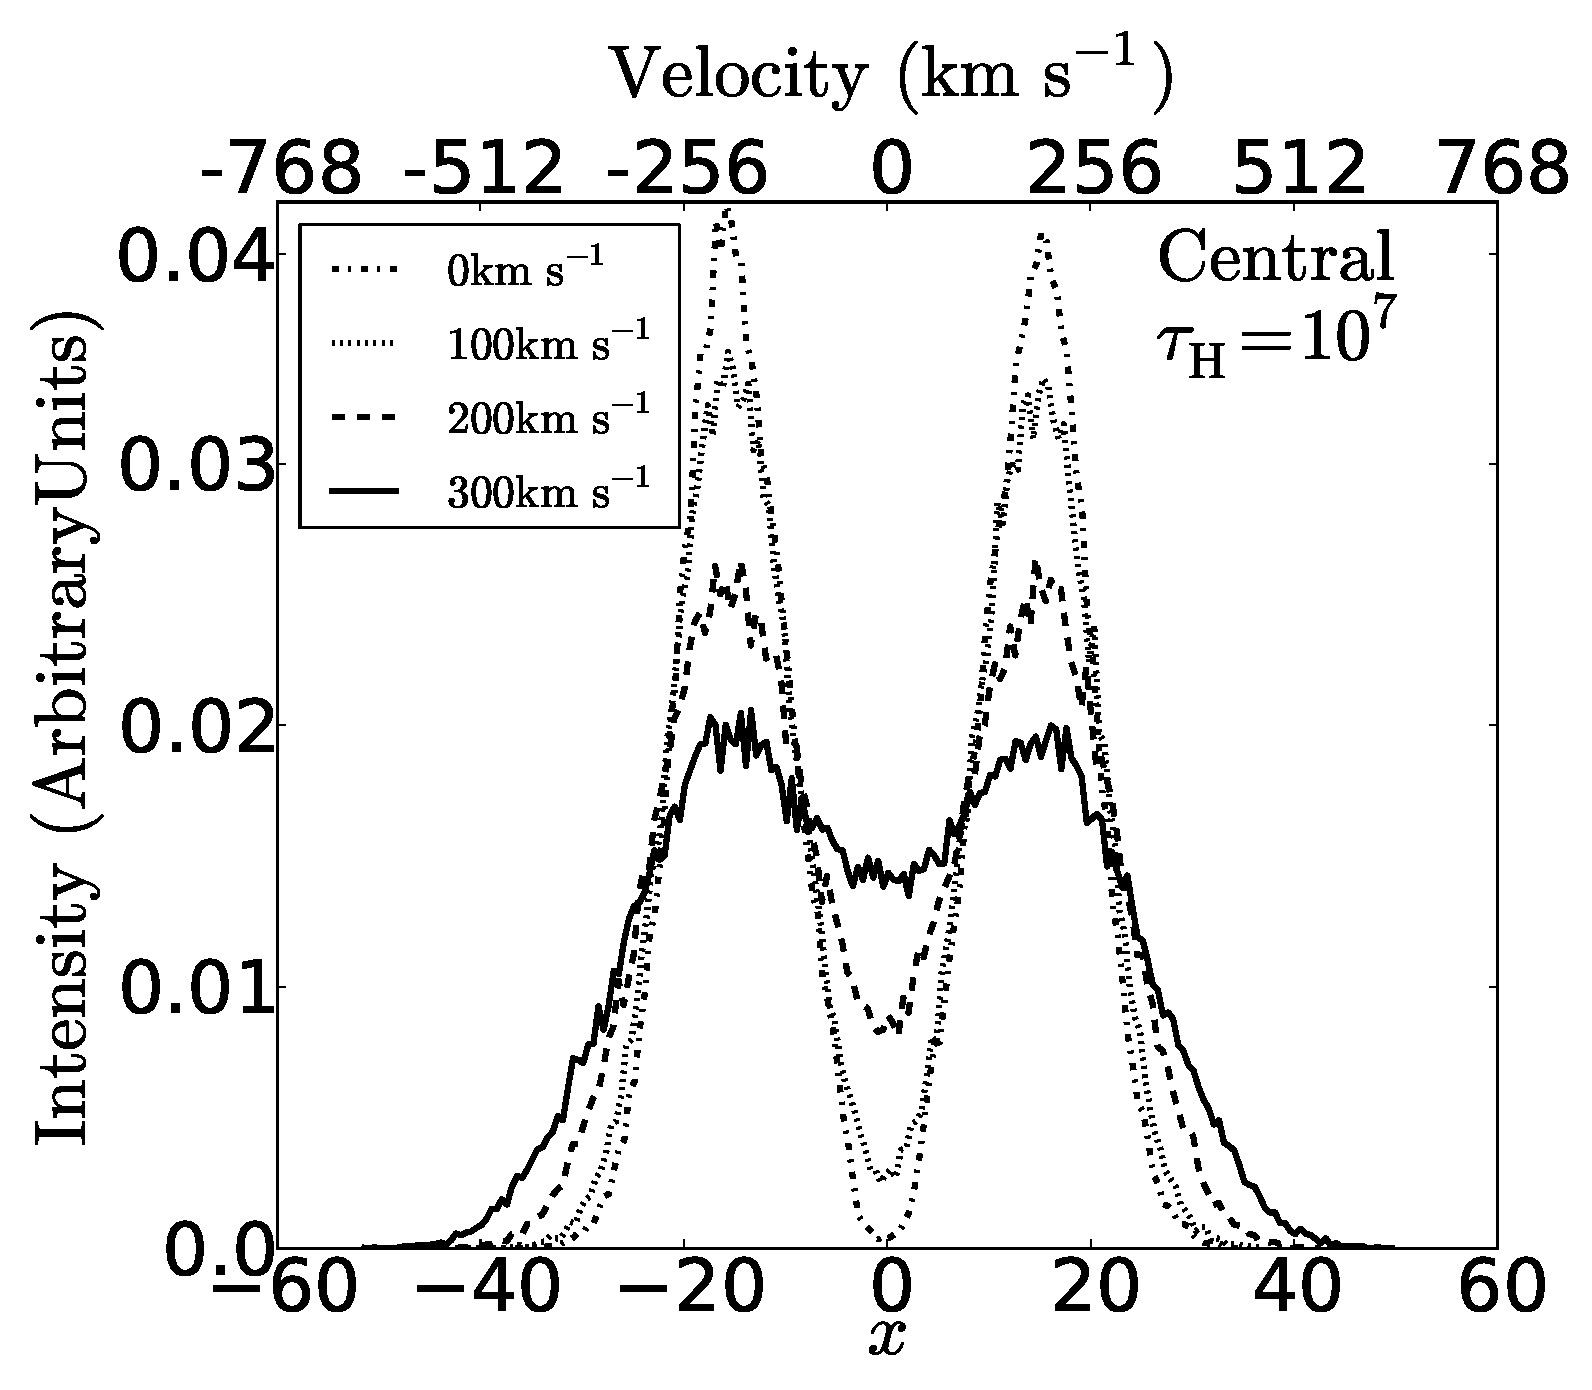
\includegraphics[width=0.45\textwidth]{f1_1.eps}
  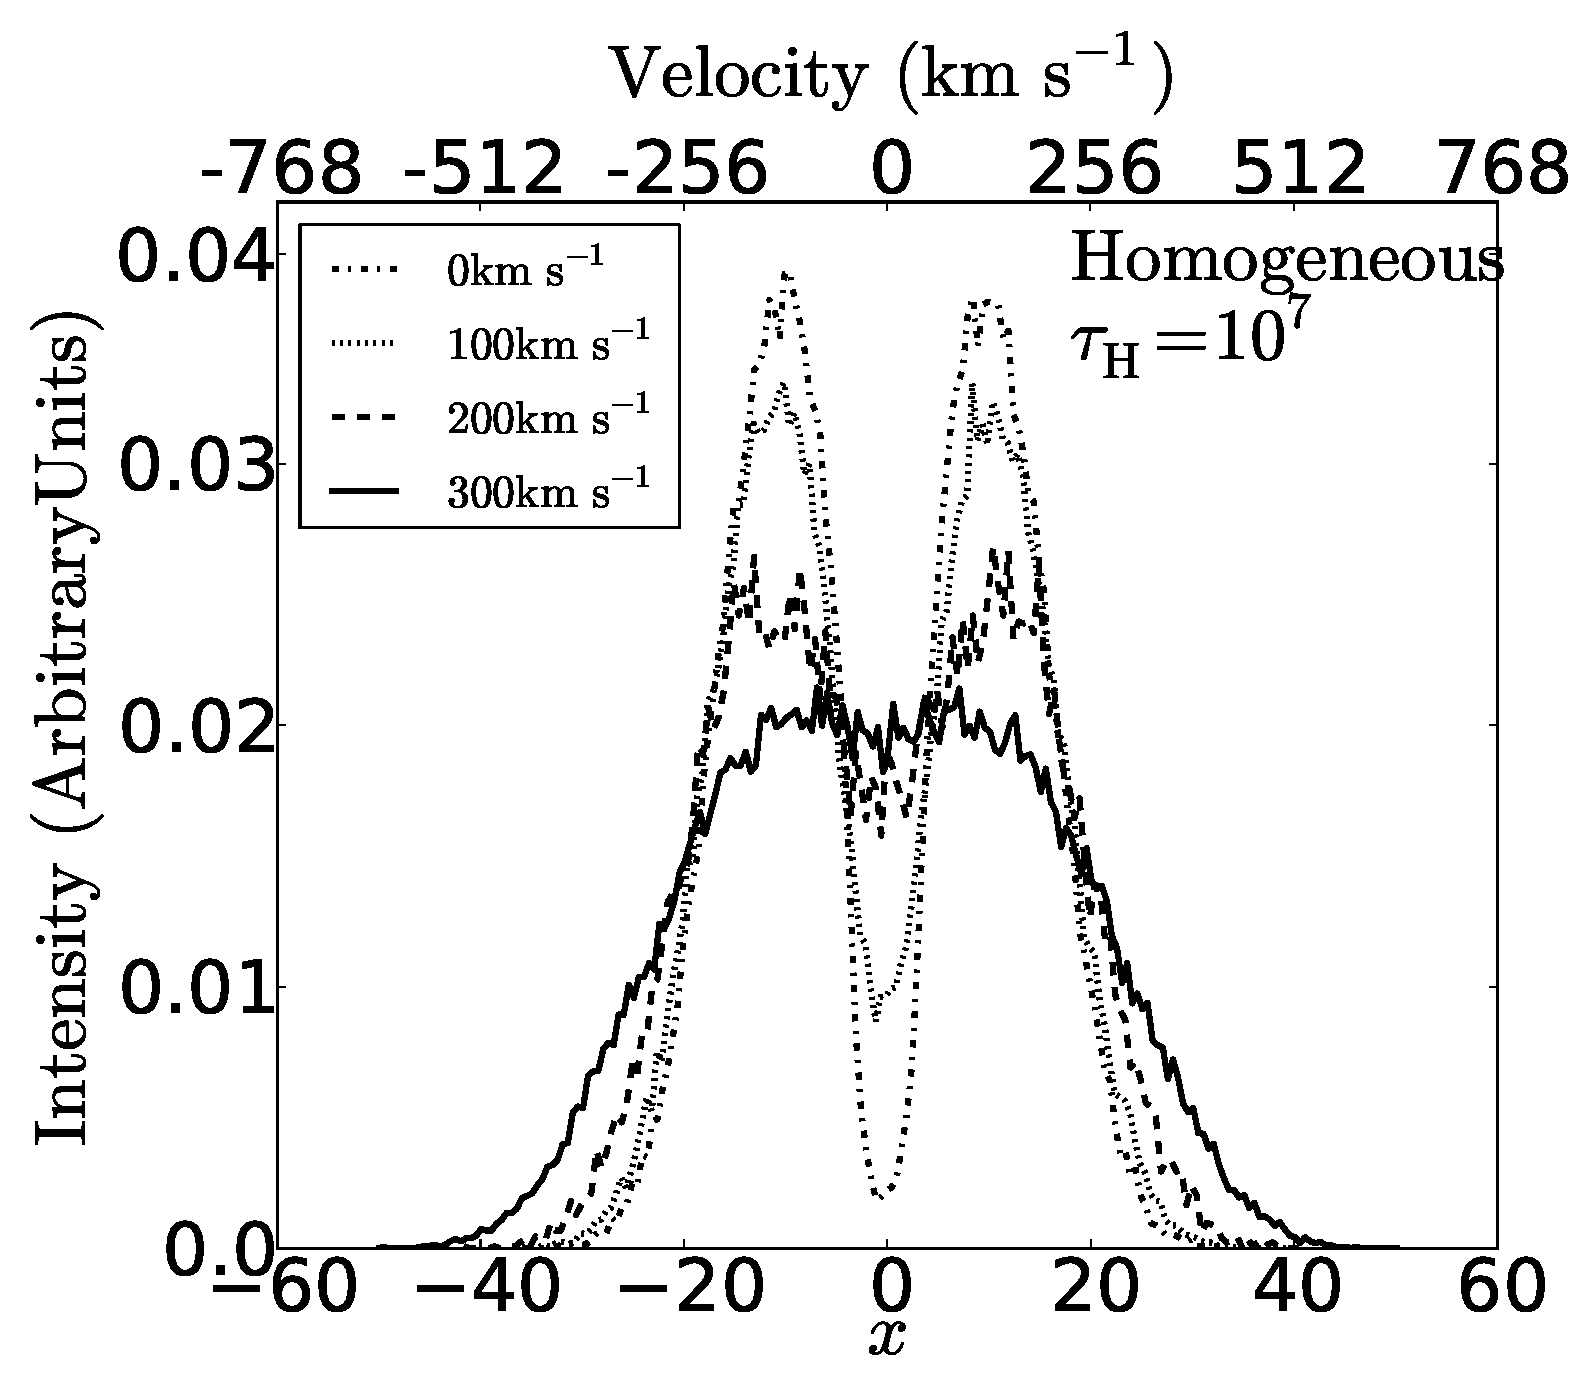
\includegraphics[width=0.45\textwidth]{f1_2.eps}
\end{center}
\caption{Shape of the \ly line for
    different velocities rotational velocities for spherical
    distributions with $\tau_{H}=10^{7}$. The left (right) panel shows
    the central (homogeneous) photon distribution. All photons were
    taken into  account regardless of their final direction of propagation.
    \label{fig:differentvelocities}}  
\end{figure*}


\subsection{Grid of Simulated Galaxies}
\label{sec:models}

In the Monte Carlo calculations we follow the propagation of $N_{\gamma}=10^5$
numerical photons through different spherical galaxies. For each galaxy
we vary at least one of the following parameters: the maximum
rotational velocity $V_{\rm max}$, the hydrogen optical depth $\tau_{H}$,
the dust optical depth $\tau_{a}$ and the initial distribution of photons
with respect to the gas. There are $60$ models initial combining all
variations of the input parameters. Table \ref{table:models}
summarizes the models.

Additionally, we have used two independently developed Monte Carlo
codes \citep{CLARA,DijkstraKramer} to perform the calculations of the
non-dusty models. The results we report are robust in the sense
that they are obtained by both codes. 

\begin{table}
\begin{center}
\begin{tabular}{llc}\hline\hline
Physical Parameter (units) & Symbol & Values\\\hline
Velocity (\kms) & $V_{\rm max}$&$0,\ 50,\ 100,\ 200,\ 300$\\
Hydrogen Optical Depth & $\tau_{H} $ & $10^{5},\ 10^{6},\ 10^{7}$\\
Dust Optical Depth & $\tau_{a}$ & $0$,$1$\\
Photons Distributions & & Central, Homogeneous\\\hline\hline
\end{tabular}
\caption{
  List of the physical parameters that define the spherical models 
  simulated in our Monte Carlo calculations. For each parameter we
  vary the values in the range listed in the last column. Taking into
  account all the possible combinations we end up with $60$ different
  models.} 
\label{table:models}
\end{center}
\end{table}


\section{Results}
\label{sec:results}

The central result of this paper is summarized in Figure
\ref{fig:differentvelocities}. It shows the evident
impact of rotation on the morphology of the emergent \ly line. Both
panels focus on the results for $\tau_{H}=10^{7}$, showing that the
influence of rotation is present both when the photons are either
homogeneously or centrally initialized over the gas volume.  

In the next subsections we characterize the line morphology by
the half-width at half intensity and the peak maxima. In order to
interpret the morphological changes in the line we also report the
median number of scatter for each \ly photon in the
simulation. For the models where dust is included we measure the 
escape fraction as a function of rotational velocity. Finally, we make
an estimate of the anisotriopic emission of the models in comparison
with static spheres.


\subsection{Line width and peak maxima}
\label{sec:widthpeak}


\begin{figure}
    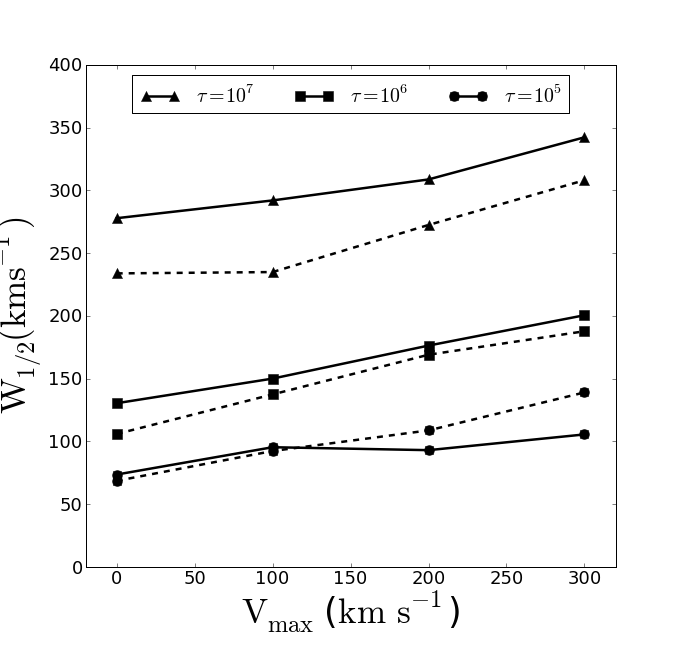
\includegraphics[width=0.45\textwidth]{NewWidthVvsVmax.eps}
    \caption{Half-width for the non-dusty models as a function of
      rotational velocity $V_{\rm max}$. Continuous (dashed) lines
      correspond to central (homogeneous) source
      distributions. \label{fig:widthvsvelocity}} 
\end{figure}


\begin{figure}
    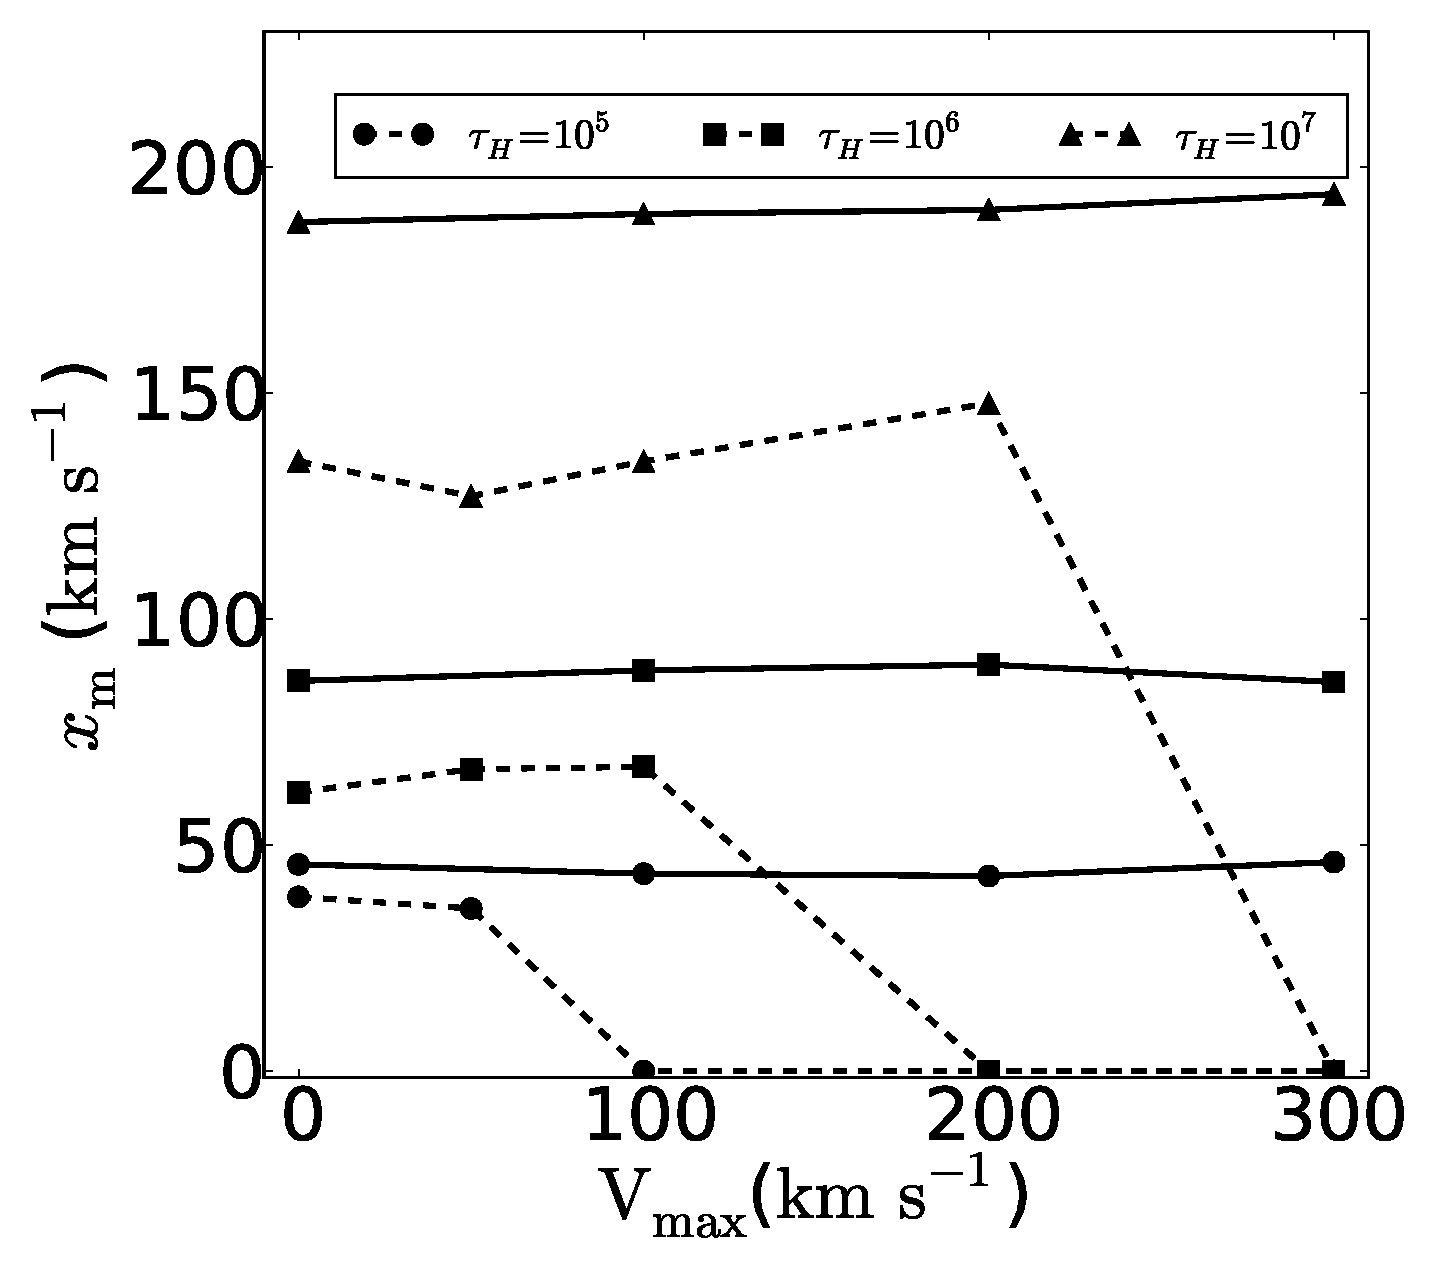
\includegraphics[width=0.45\textwidth]{f3.eps}
\caption{Position of the peak maxima as a function of rotational
  velocity $V_{\rm max}$. Continuous (dashed) lines correspond to
  central (homogeneous) source distributions. A value of $x_{\rm
    max}=0$ indicates that line becomes single
  peaked. \label{fig:maximumsvsvelocity}}  
\end{figure}

There are three clear effects on the line's morphology as the
rotational veloctiy increases. First, the line
broadens; second, the double peaks reduce their intensity; and third,
the intensity at the line center rises. The two last effects give the
impresion that the double peaks are merger into one at high rotational
velocities, a result that is evident for the homogeneously distributed
sources as shown in right panel in Figure \ref{fig:differentvelocities}.

We use the full width at half maximum (FWHM), $W$, to quantify the line
broadening. Figure \ref{fig:widthvsvelocity} shows how $W$ increases
with rotational velocity. {\bf Here we need to check the numbers to
  say something more specific.}

We parameterize the dependency of the linewidth as $W^2 =
W_{0}^2 + V_{\rm max}^2/\lambda^2$, where $W_{0}$ is the
velocity width in the static case and $\lambda$ is a positive
scalar to be determined as a fit to the data. With this test we want
to know to what extent the new velocity witdth can be expressed as a
quadratic sum of the two relevant velocities in the problem. We find
that for $\lambda = x\pm y$ ($\lambda=x\pm y$) for the central
(homogeneous) sources.

In order to quantify the transition to a single peak we measure the
position for the peak maxima as a function of the rotational
velocity. Our results are presented in Figure
\ref{fig:maximumsvsvelocity} where it is clear that for central
sources there are always two peaks with fixed positions as the rotational
velocity changes. However, in the case of homogeneously emitted
sources the maxima position remain close to constant until some
velocity threshold the line becomes single peaked with $x_{\rm m}=0$
\kms. {\bf By inspection we find that in all cases the transition has
occurred when the rotational velocity is larger than the intrinsic
linewidth OR HALF WIDTH ONCE THE NUMBERS ARE FIXED?}.

One possible explanation for the emergence of the single peak in the
homogeneous source systems is that some photons close to the surface
(a sort of photosphere) can escape with a low number of scatterings,
allowing them to stay close to the line's center. Increasing the
rotational velocity $V_{\rm max}$ reduces the optical depth making the
photosphere region effectively larger, increasing the number of
photons escaping close to the line's center. 

However, for the central emission the transition to a single peak is
never completed in the range of explored parameters. The absence
of a single peak phase could be partially explained by the absence of a
photosphere, in this case the average number of scatterings to escape
should remain close to constant as the rotational velocity
increases. The rise in intensity at the line's center could instead
mean that the scattering in a medium with bulk motion are inefficient
in driving photons outside that frequency region.

In order to explore our interpretation for these two scenarios we now 
quantify the effect of rotation on the number of scatterings.

\subsection{Average Number of Scatterings}


\begin{figure}
    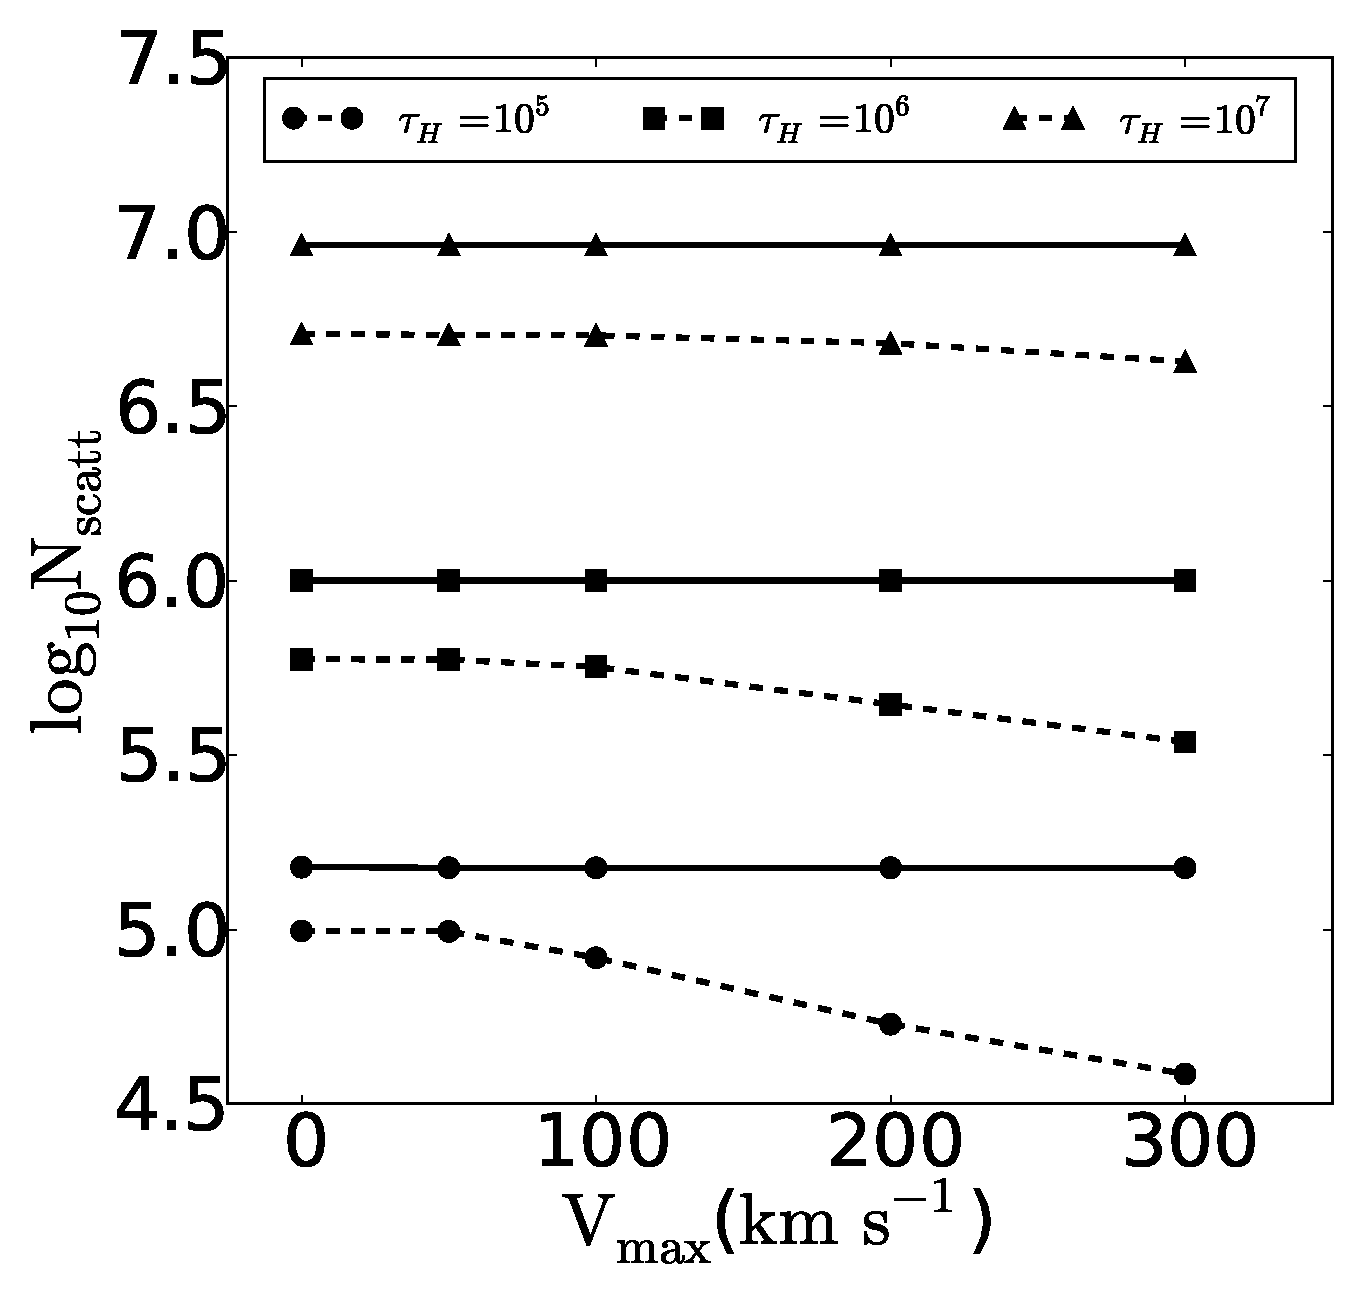
\includegraphics[width=0.45\textwidth]{f4.eps}
\caption{Logarithm of the average number of scatterings as function of
  rotational velocity. Continuous (dashed) lines represent an
  central (homogeneous) distribution of sources. \label{fig:Nscatt}}    
\end{figure}


\begin{figure*}
\begin{center}
  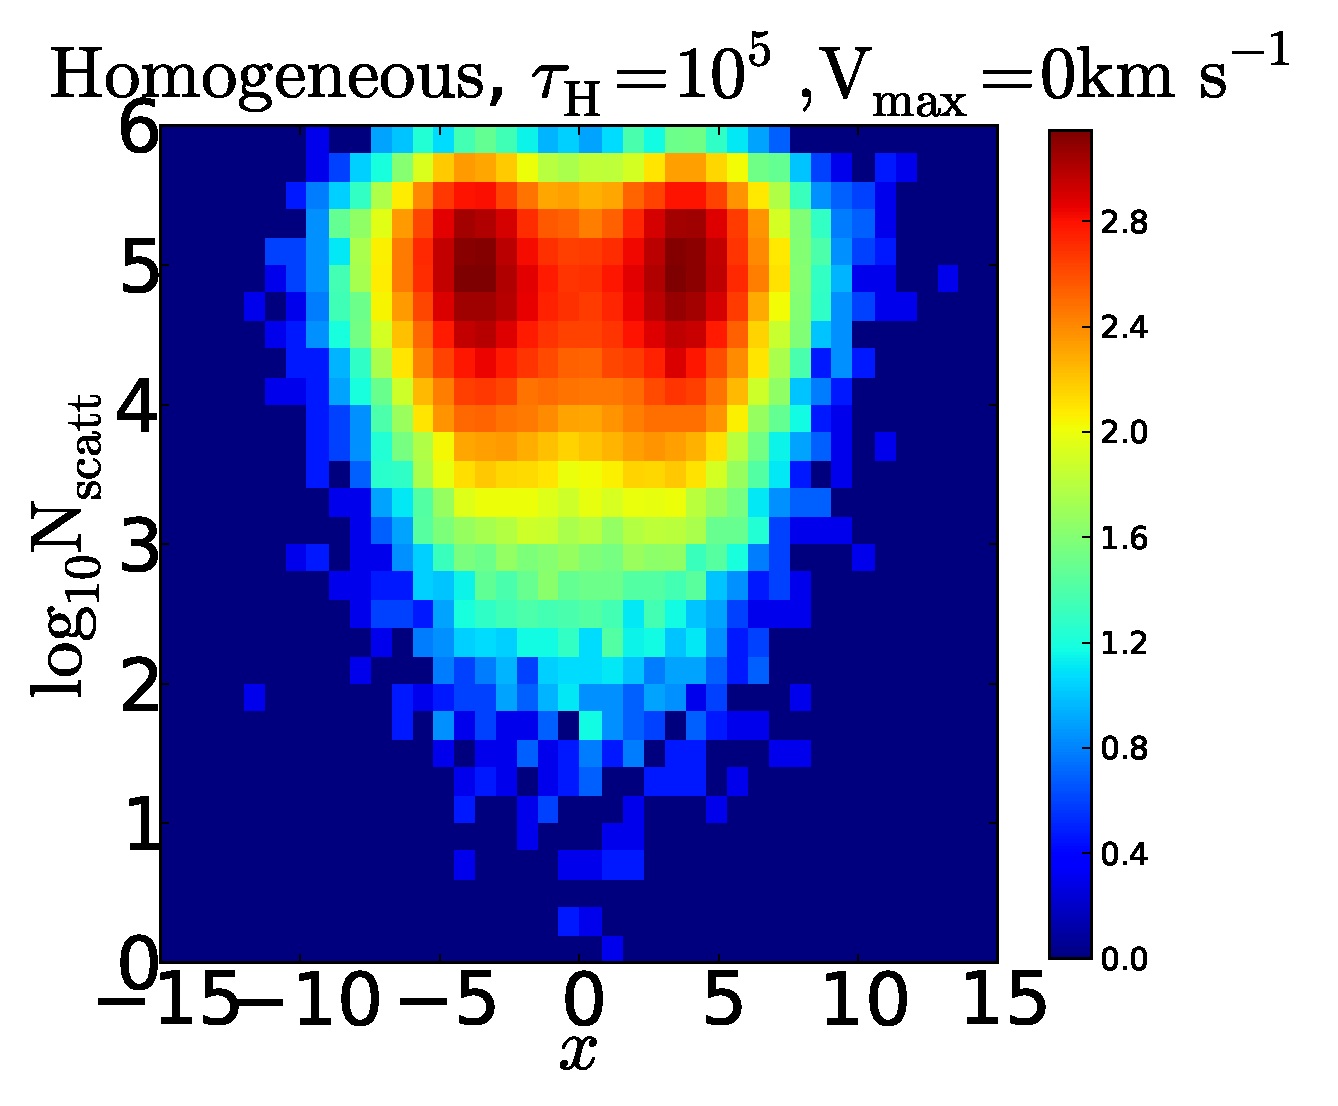
\includegraphics[width=0.45\textwidth]{f5_1.eps}
  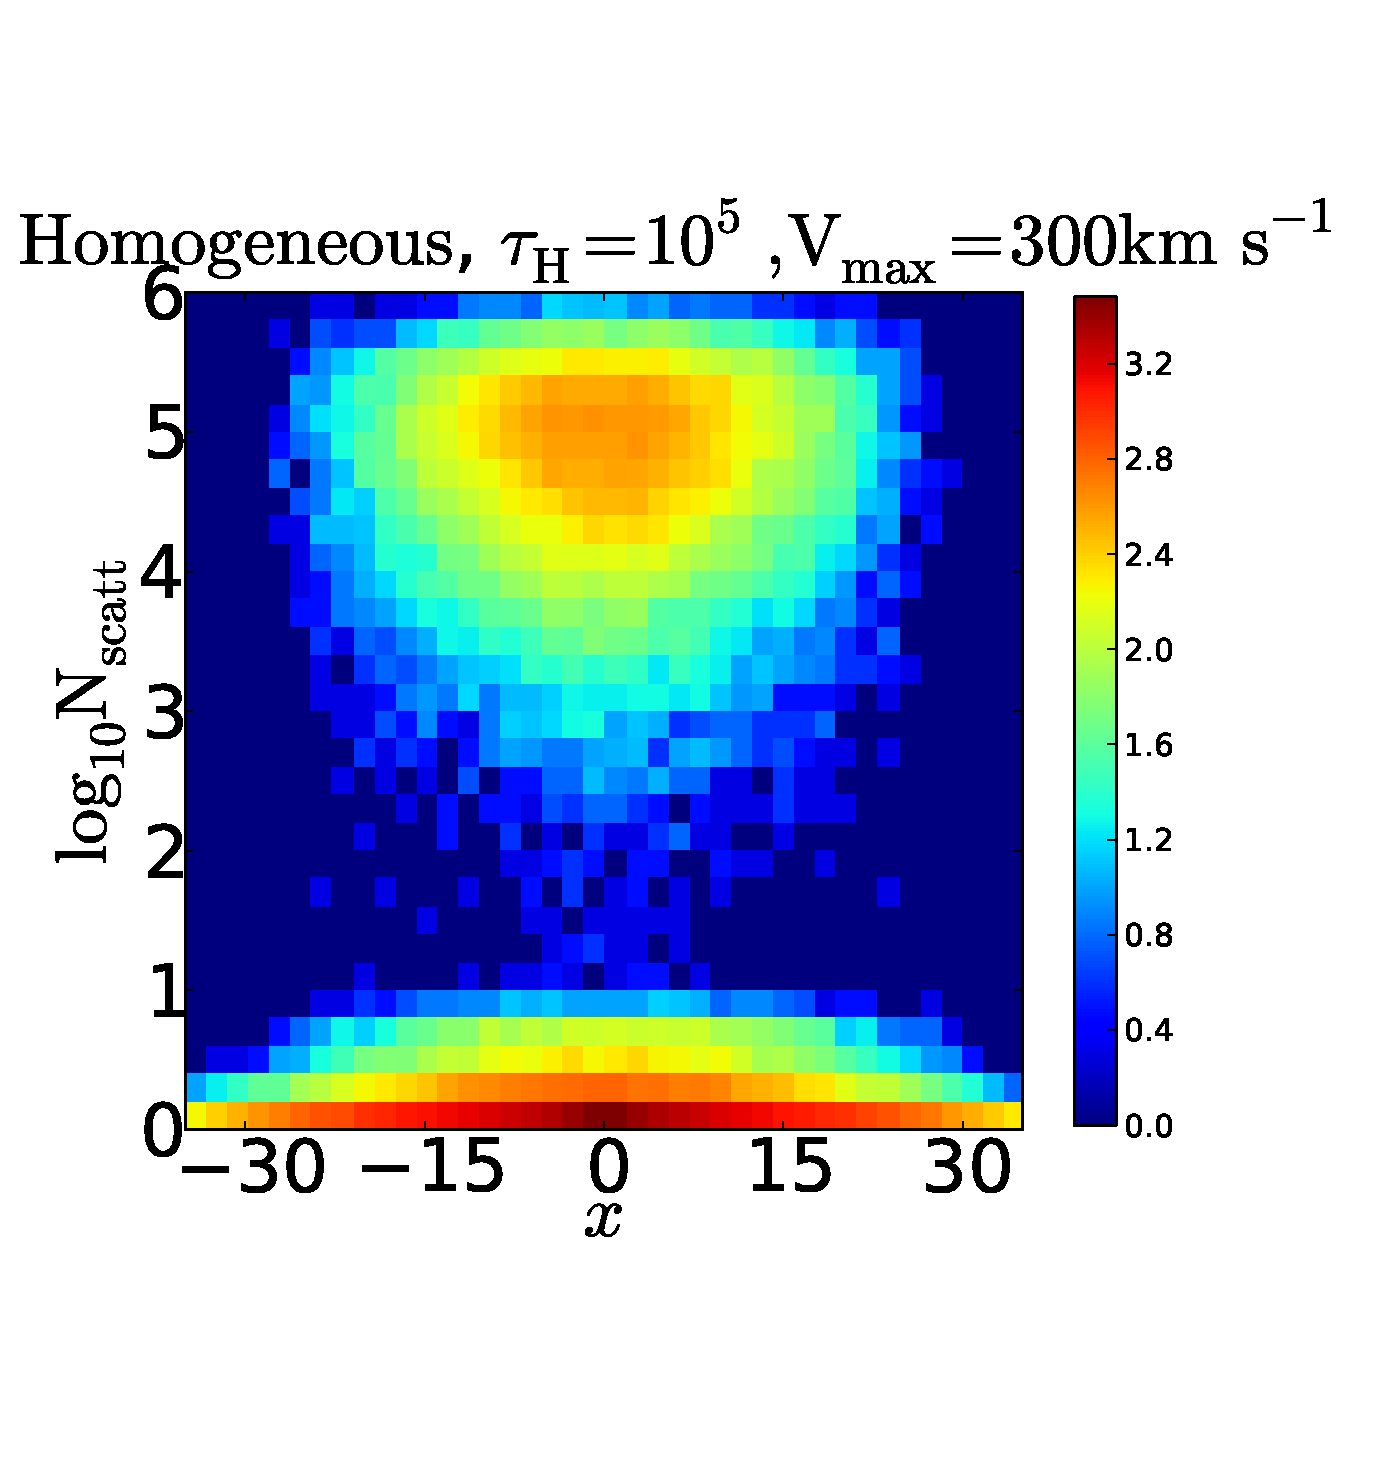
\includegraphics[width=0.45\textwidth]{f5_2.eps}
  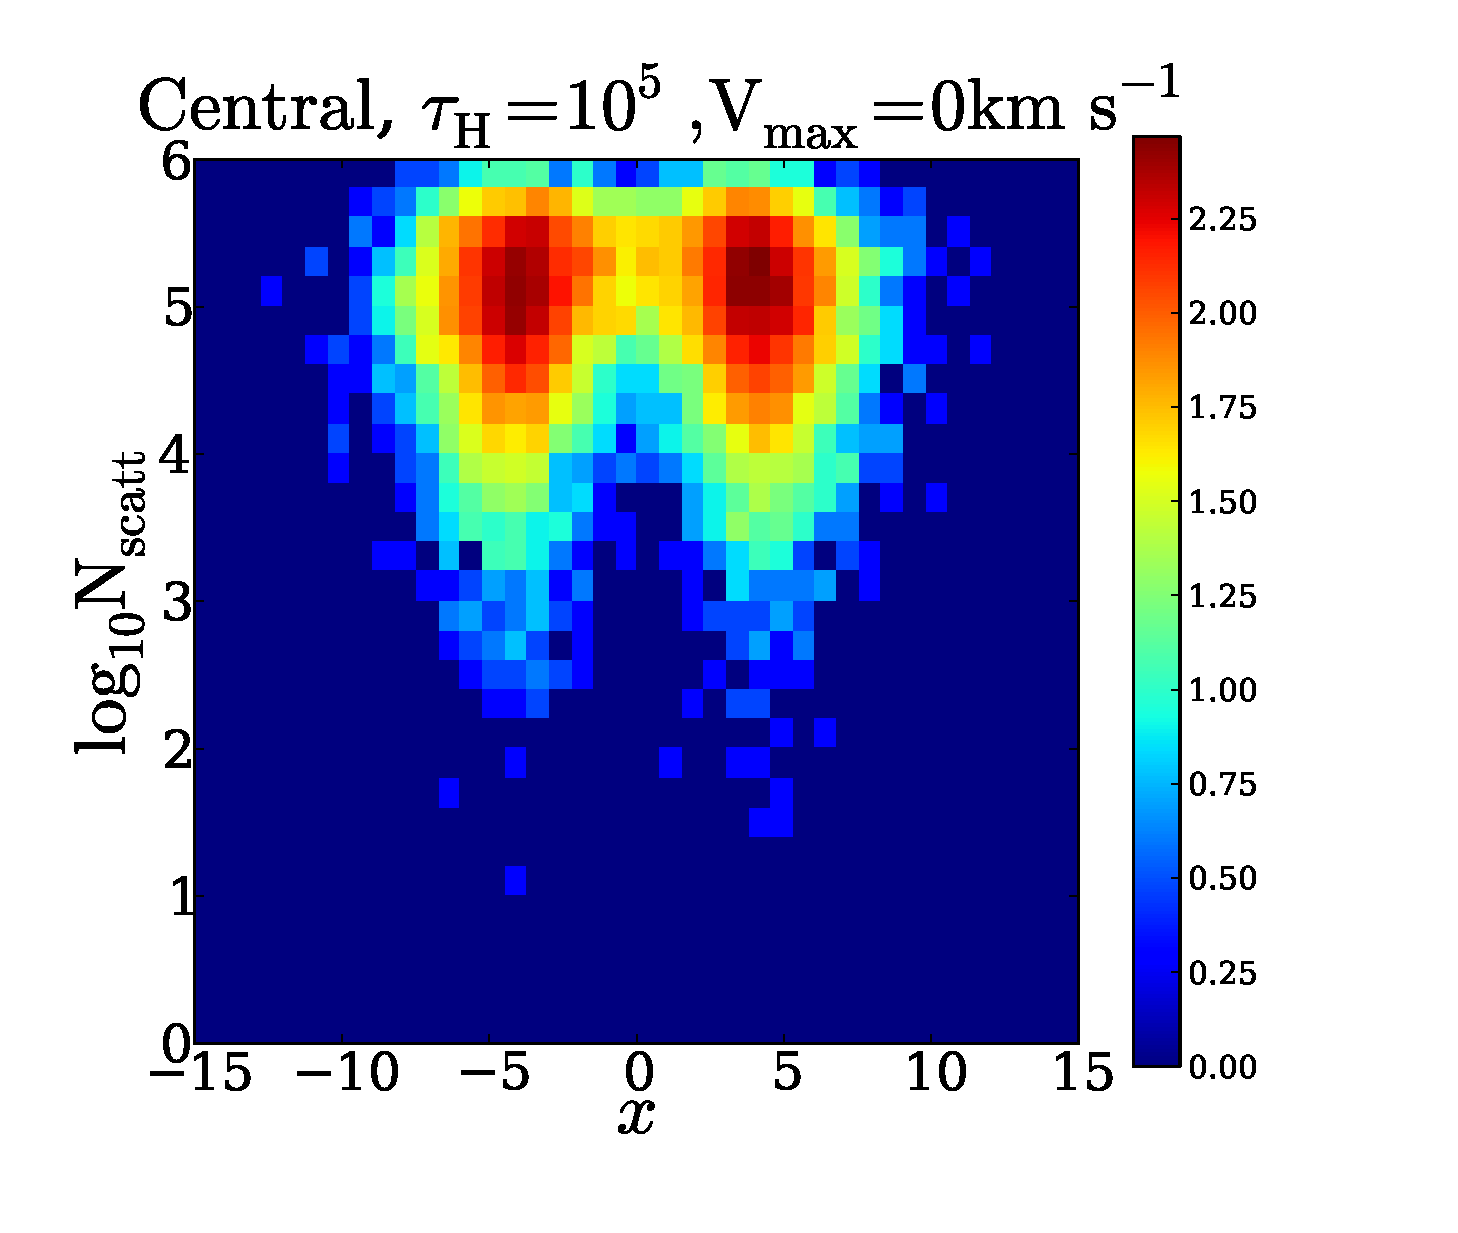
\includegraphics[width=0.45\textwidth]{f5_3.eps}
  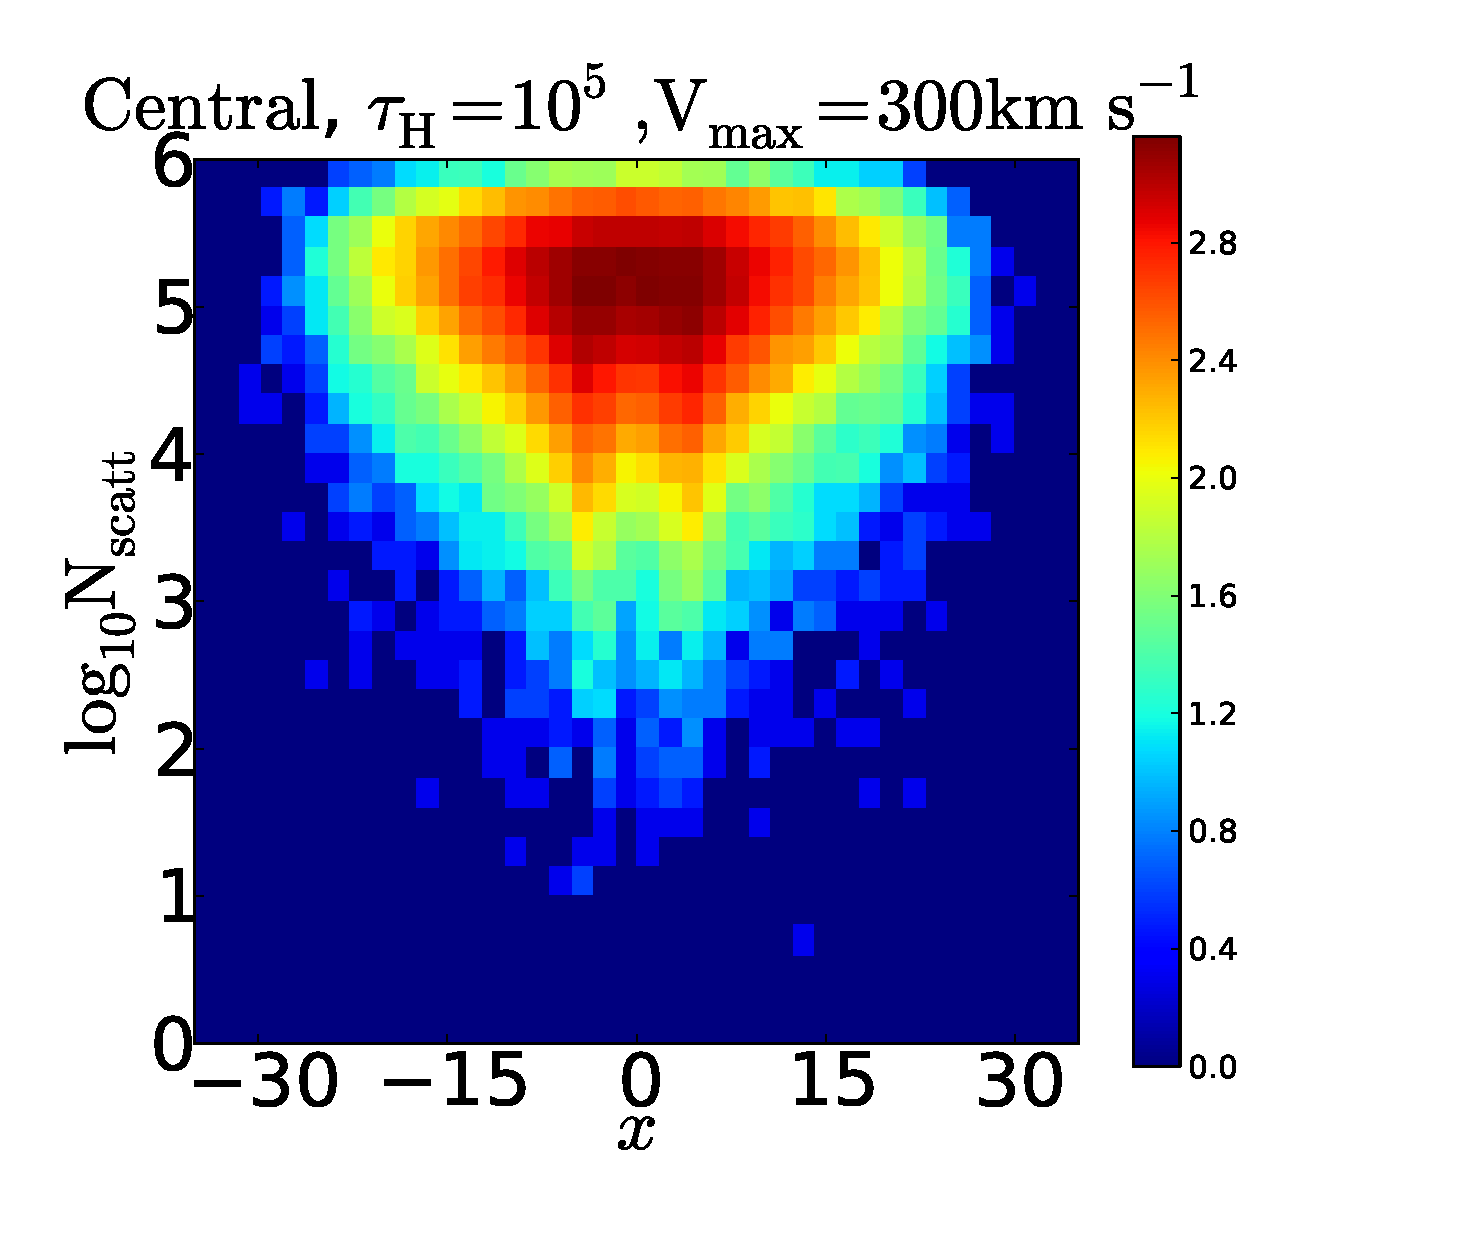
\includegraphics[width=0.45\textwidth]{f5_4.eps}    
\end{center}
    \caption{2D histogram of $N_{\rm scatt}$ vs $x$. The upper (lower) panels
      show the homogeneous (central) source distribution. Left
      corresponds to the static case and right
      $V_{\rm max}=300\kms$. The color scale is logarithmic on the
      number of photons with given values of $N_{\rm scatt}$ and
      $x$. \label{fig:Nscatt2D}}   
\end{figure*}

The number of scatterings affects the escape frequency of a \ly photon.
In static cases, a large value of the optical depth correlates with a
high number of scatterings, increasing the probability of finding a
\ly photon far from the line's center. As a result the peak maxima
shifts from the center as the amount of neutral hydrogen
increases. This can be precisely quantifyied in the static slab
with central sources where the maxima position are related to
the optical depth and the temperature as $x_{m}=\pm 1.066(a\tau_{\rm
  H})^{1/3}$ \citep{Harrington73}. In the same model the average
number of scatterings depends only on the optical depth $\langle
N_{\rm  scatt}\rangle=1.612\tau_{\rm   H}$
\citep{Adams72,Harrington73}, in the case of homogeneously distributed
sources $\langle N_{\rm   scatt}\rangle=1.16\tau_{\rm   H}$
\citep{Harrington73}.   



In Figure \ref{fig:Nscatt} we show the average number of scatterings
$\langle N_{\rm scatt}\rangle$ as a function of the rotational velocity
$V_{\rm max}$. For the central source distribution the average number of
scatterings $\langle N_{\rm   scatt}\rangle$ changes less than $0.5\%$
for different velocities. In this setup the number of scatterings is
proportional to the optical depth, with $\langle N_{\rm
  scatt}\rangle= (1.50, 1.00, 0.92)\tau_{\rm   H}$ for optical depth
values of $\tau_{\rm H} = (10^{5}, 10^{6}, 10^{7})$, respectively


From Figure \ref{fig:Nscatt} is also clear that for the homogeneous
distribution there is a clear decrease of $\langle N_{\rm
  scatt}\rangle$ as the $V_{\rm max}$ increases. For instance, for
$\tau_{\rm H}=10^5$ the average number of scatterings decreases by
$61\%$ at $V_{\rm max}=300\kms$ in comparison to the static case.  

In this case we find that for a static sphere $\langle N_{\rm
  scatt}\rangle= (0.99, 0.59, 0.51)\tau_{\rm   H}$, this
representsfactors of $(0.66, 0.59, 0.55)$ lower than the centrally
emitted photons. In contrast the analytic solution for the homogeneous
slab gives $0.72$ times less scatterings in the homogeneous case than
in the central one. 

In order to gain a deeper understanding of these results and explain
the results for the maxima in the line morphology we make 2D
histograms for the number of scatterings as a function of the outgoing
dimensionless frequency $x$. In Figure \ref{fig:Nscatt2D} we show
such histogram in the case $\tau_{\rm H}=10^5$ for the
static case and $V_{\rm max}=300$\kms. The upper (lower) panels show the
results for the homogeneous (central) source distribution. The color
scale is logarithmic in the number of photons at a certain value
$x$-$N_{\rm scatt}$. 

The top right panel of Figure \ref{fig:Nscatt2D} (homogeneous sources,
high rotational velocity) supports our hypothesis about
the photo-sphere in the homogeneous distribution. In this case most of
the photons that left with $x\sim 0$ have escaped with less than $10$
scatterings. This also explains the decrease in the average number of
scatterings observed in Figure \ref{fig:Nscatt}.

However, for a central distribution the situation is quite different
(lower panels). In this case the number of scatterings remains high,
in the order of the optical depth, but the two peaks do get closer to each
other. Here the most probable physical picture is that each
scattering, due to the bulk velocity of the gas, is inefficient in
driving the photon outside the line center.



\subsection{Dusty Clouds: Escape Fraction}
\label{sec:escapefraction}

\begin{figure}
  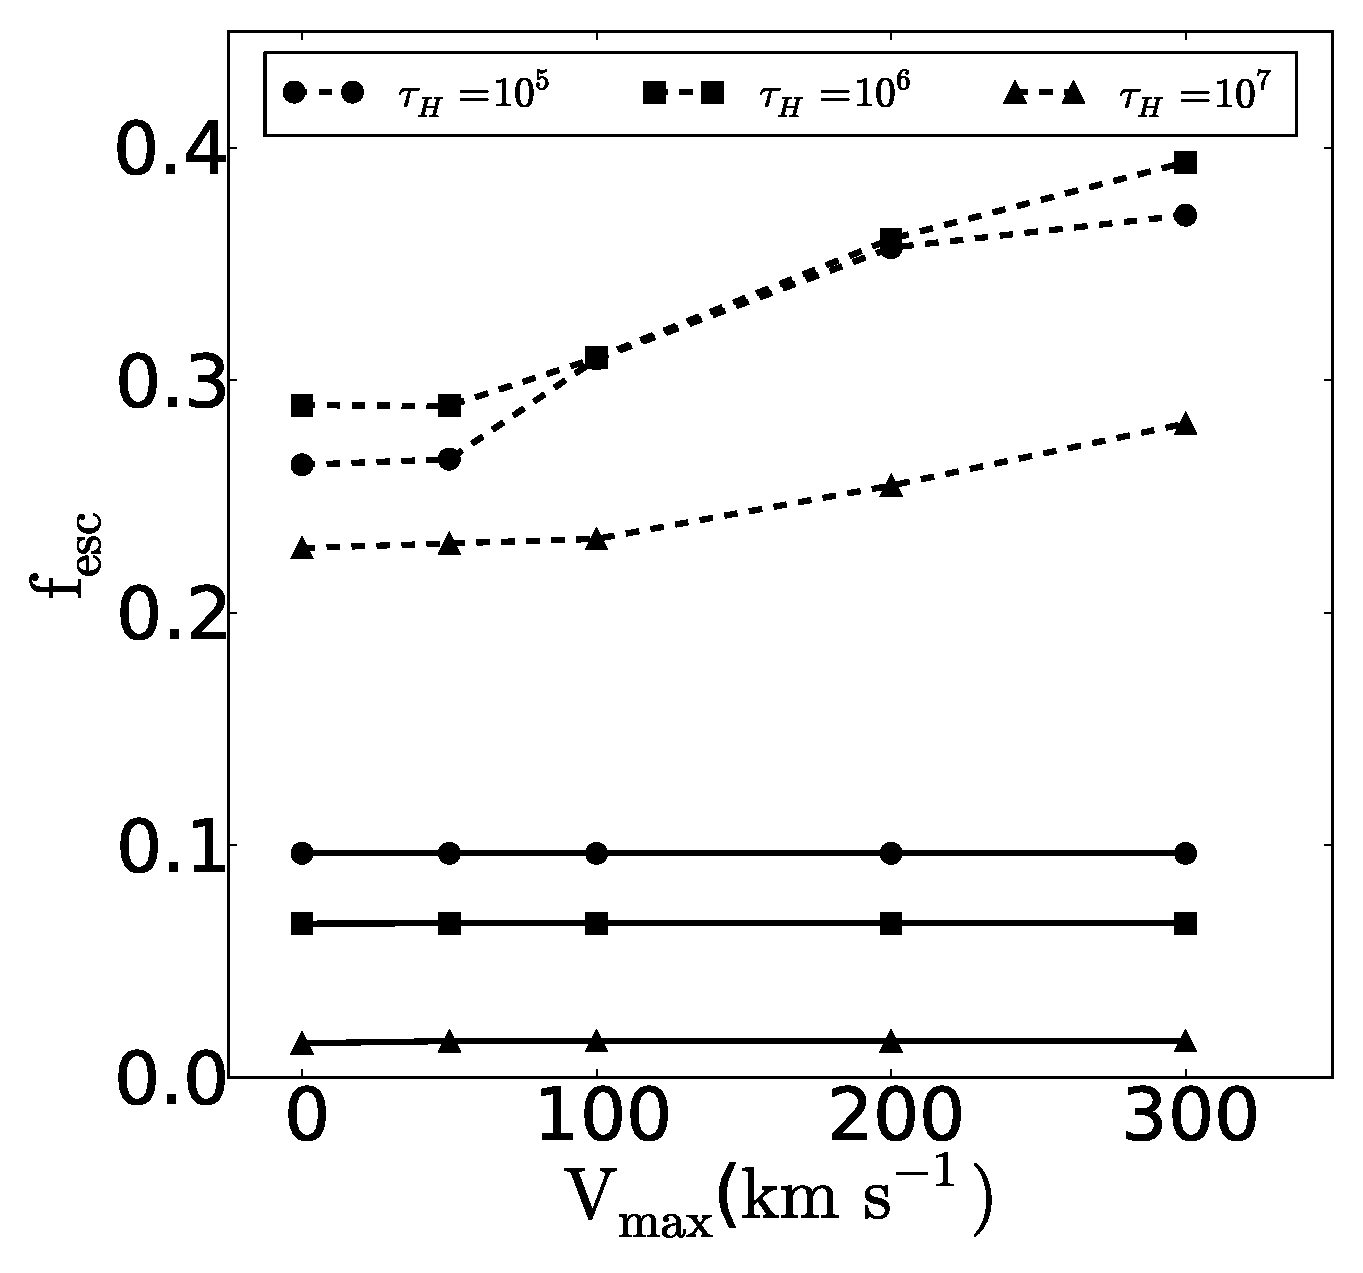
\includegraphics[width=0.45\textwidth]{f6.eps}
  \caption{Escape fraction as a function of rotational velocity. All
    these models have $\tau_{a}=1$. The continuous (dashed) lines
    correspond to central (homogeneous) models.
    \label{fig:efvsv}}
\end{figure}


\begin{figure}
  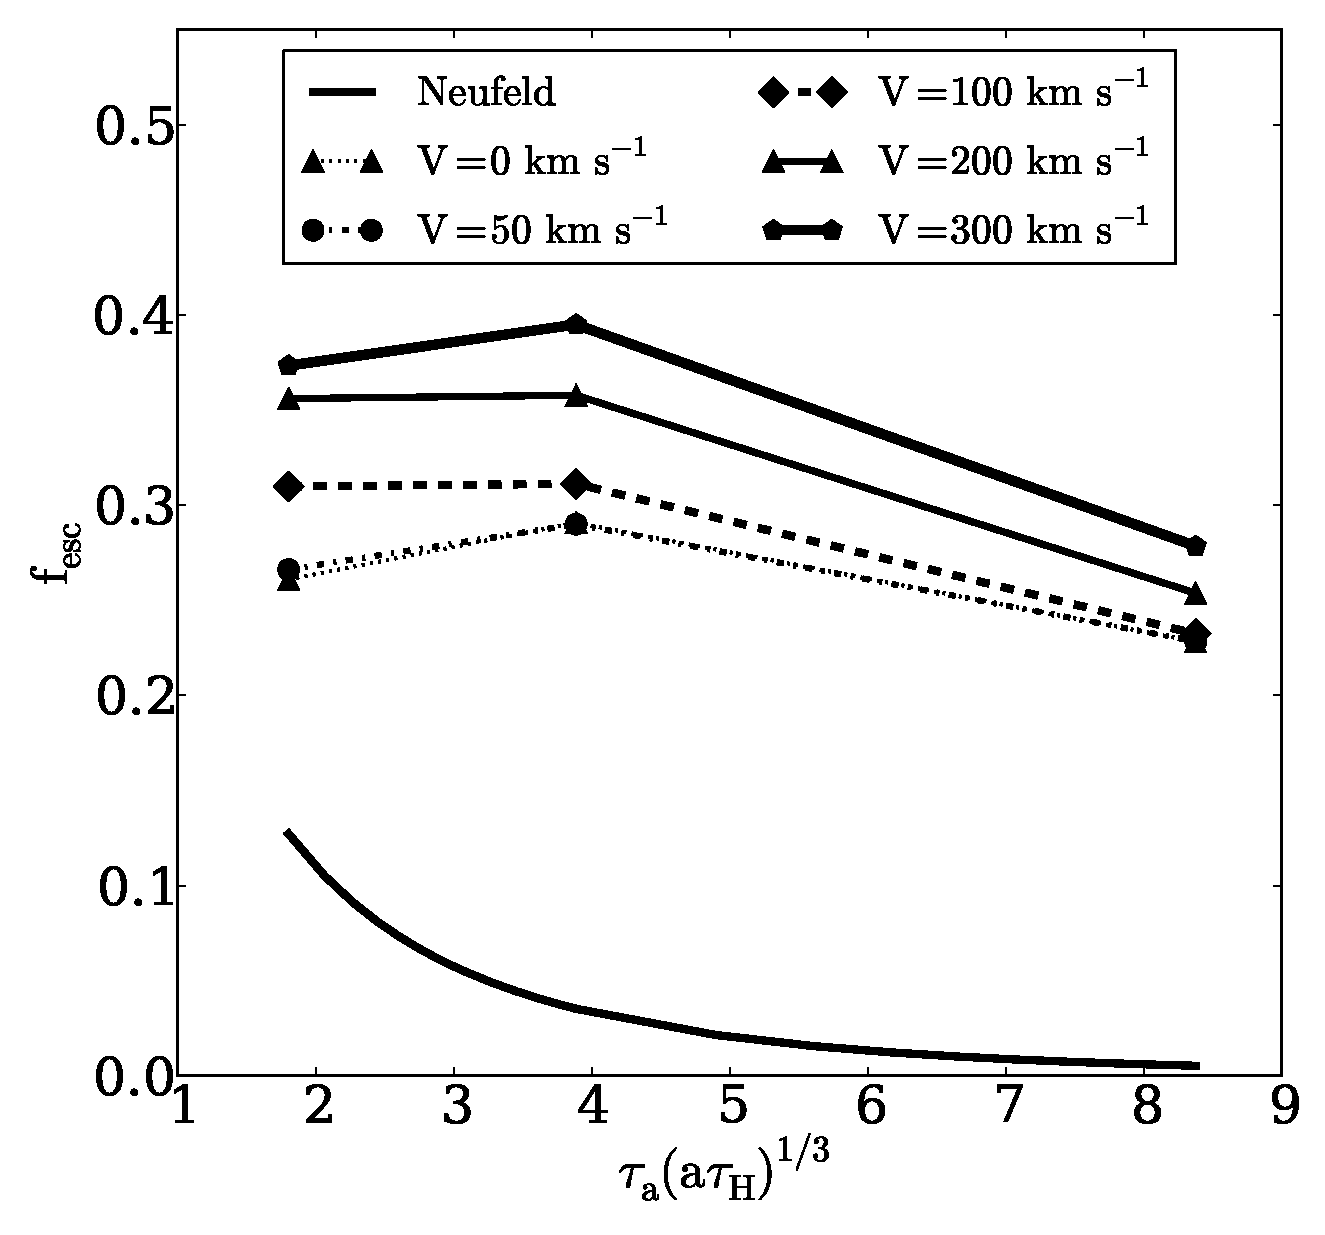
\includegraphics[width=0.45\textwidth]{f7.eps}
  \caption{Escape fraction as a function of the
    product $(a\tau_{\rm H})^{1/3}\tau_{a}$. The analytic solution for
    the infinite slab is shown as a continuous line. Different dashed
    lines correspond to different rotational velocities.
    {\bf IS THE ALBEDO TAKEN INTO ACCOUNT?}
    \label{fig:efvsNeufeld}}   
\end{figure}


In the case of dusty clouds, all changes in the average number
of scatterings presented in the previous subsection have a direct
bearing on the escape fraction. From the results we have just obtained
we can predict that for central source distributions the escape
fraction will barely change, while larger effects should be expecte
for homogeneously distributed sources. 

Figure \ref{fig:efvsv} confirm these expectations. It shows the escape
fraction as a function of the rotational velocity. The curves for the
central source distribution stay flat, while for the homogeneous case
there is a clear rise with rotational velocity.  Rotation has a higher relative impact in
the models with low optical depth. For instance, in models with
$\tau_{\rm H}=10^5$, the static scape fraction is $0.26$ and increases
to $0.37$ for $V_{\rm max}=300$ \kms. Table \ref{table:escape} lists
all the values for the escape fraction {\bf We also need a table
  listing the escape  fraction values.}  

In Figure \ref{fig:efvsNeufeld} we put these results in the context of
the analytic solution for the infinite slab \citep{Neufeld90}. In
Neufeld's set-up the analytic solution depends uniquely on the product
$(a\tau_{\rm   H})^{1/3}\tau_{a}$, an approximation that is valid only
in the limit $a\tau_{\rm   H}\gg 1$. The dashed lines in Figure
\ref{fig:efvsNeufeld} show the results for the different rotational
velocities. First of all we note that the escape fraction does not
increase from $\tau_{\rm H}=10^{5}$ to $\tau_{\rm H}=10^{6}$, a fact
that is explained since there is a transition from a opaque to an extremely opaque medium
which affect affects how \ly photons escape from the medium: single flight 
vs. single excursion. {\bf Que quiere decir eso de single flight y
  single excursion, porque explica eso la fraccion de escape?} 
 %we are in a regime where the condition for the analytic expectations
 %($a\tau_{h}\gg 1$) does not hold.  

\subsection{Anisotropy and off-centered emission}

\label{sec:off-center}
\begin{figure}
  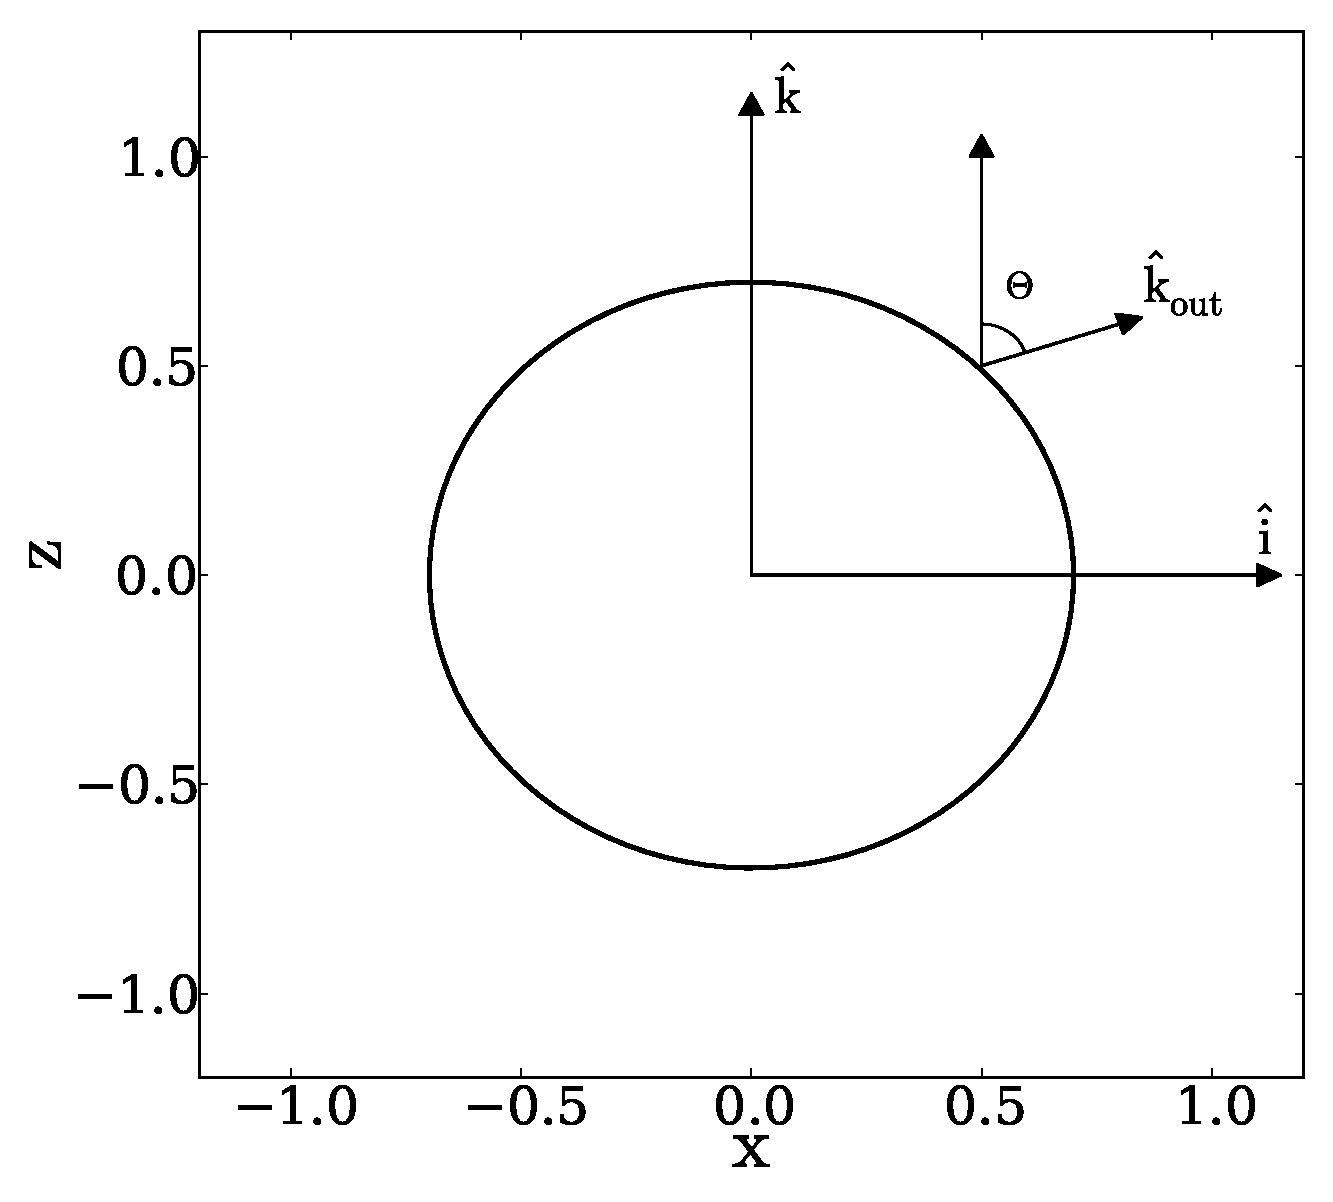
\includegraphics[scale=0.3]{f8.eps}
  \caption{The two small circles show the two different spherical
    off-centered emitting regions with respect to the larger spherical
    gas distribution. The angular velocity vector is
    defined to be along the $\hat{\i}$ direction (outwards the
    page). In order to study a possible anysotropy we place an
    observer along the the $\hat{\j}$ direction. The vector
    $\hat{k}_{\rm out}$ represents the outgoing direction of an
    escaping \ly photon. {\bf Si el observador esta en j, entonces las
    dos esferas no deberian estar sobre el eje k? Lo mejor es ademas
    hacer las dos circulos pequenos punteados. Por otro lado, como se
    habian definido las velocidades, el eje de rotacion es el eje k}
    \label{fig:OCspheres}} 
\end{figure}

\begin{figure}
  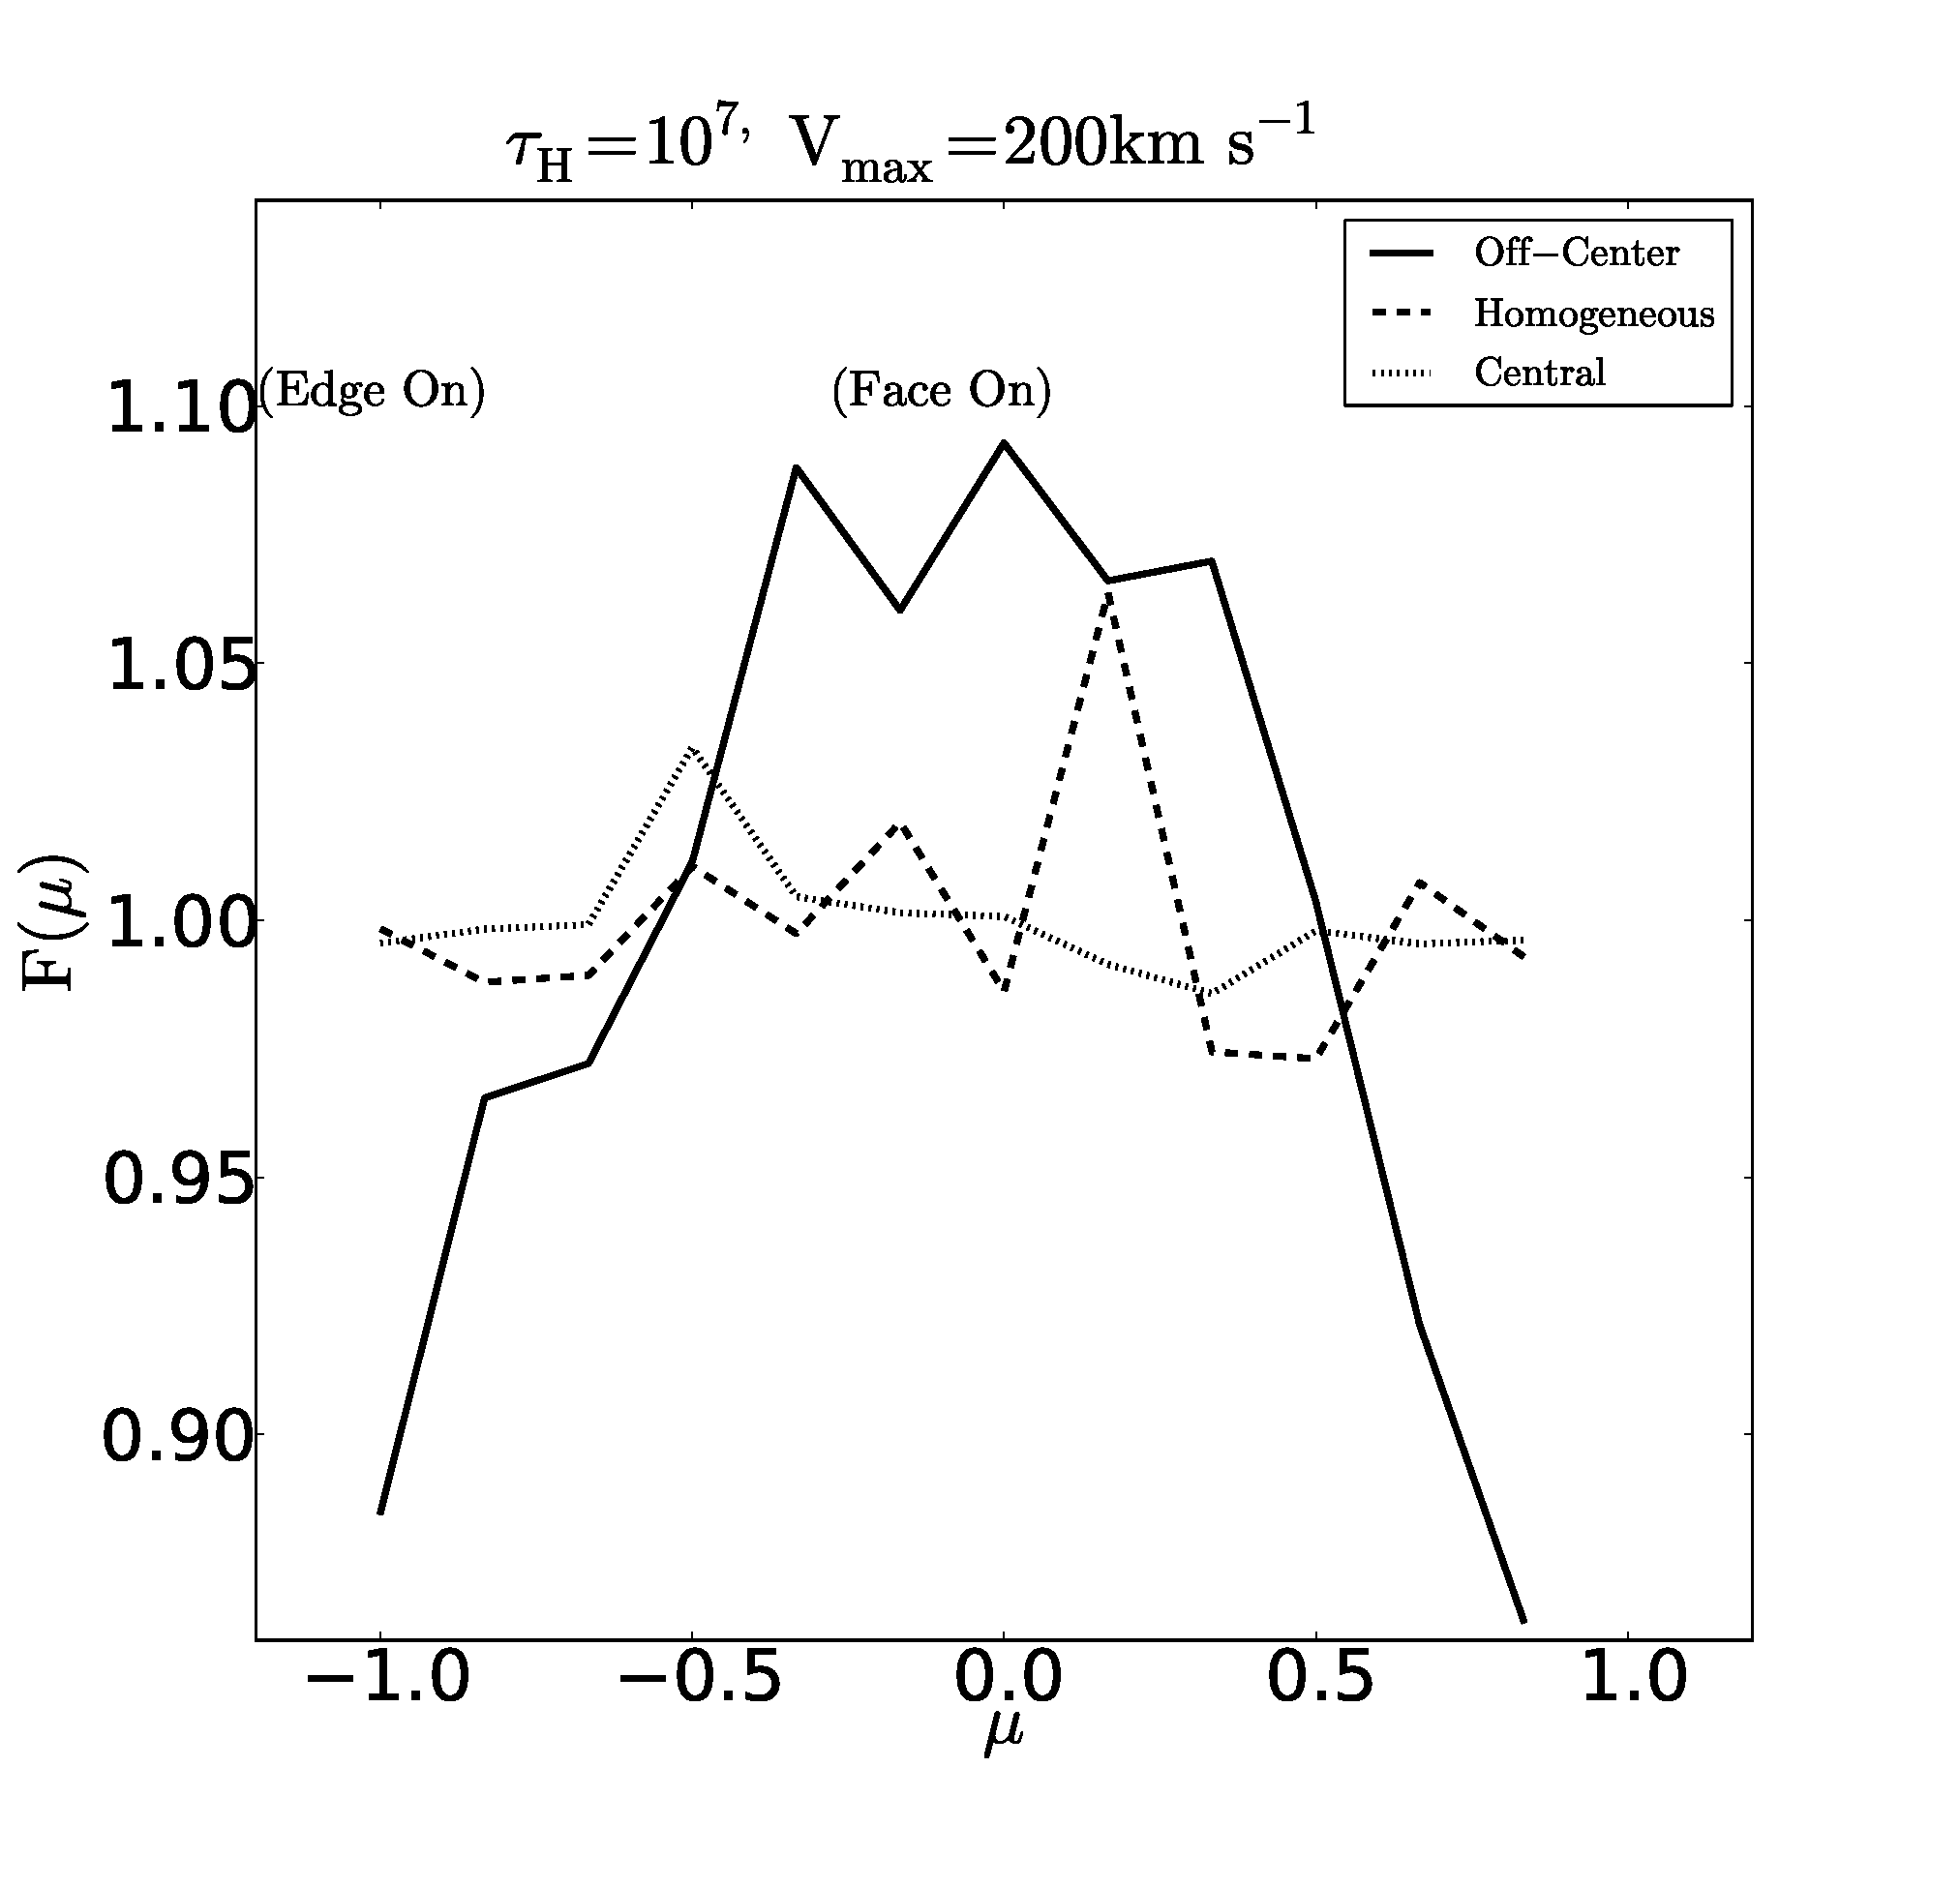
\includegraphics[scale=0.35]{f9.eps}
  \caption{$\mu$ histogram showing the orientation effects for the different
  distributions central(Points line), homogeneous(Dashed) and off-Center(Solid line).  
    \label{fig:muhisto}} 
\end{figure}



\begin{figure*}
\begin{center}
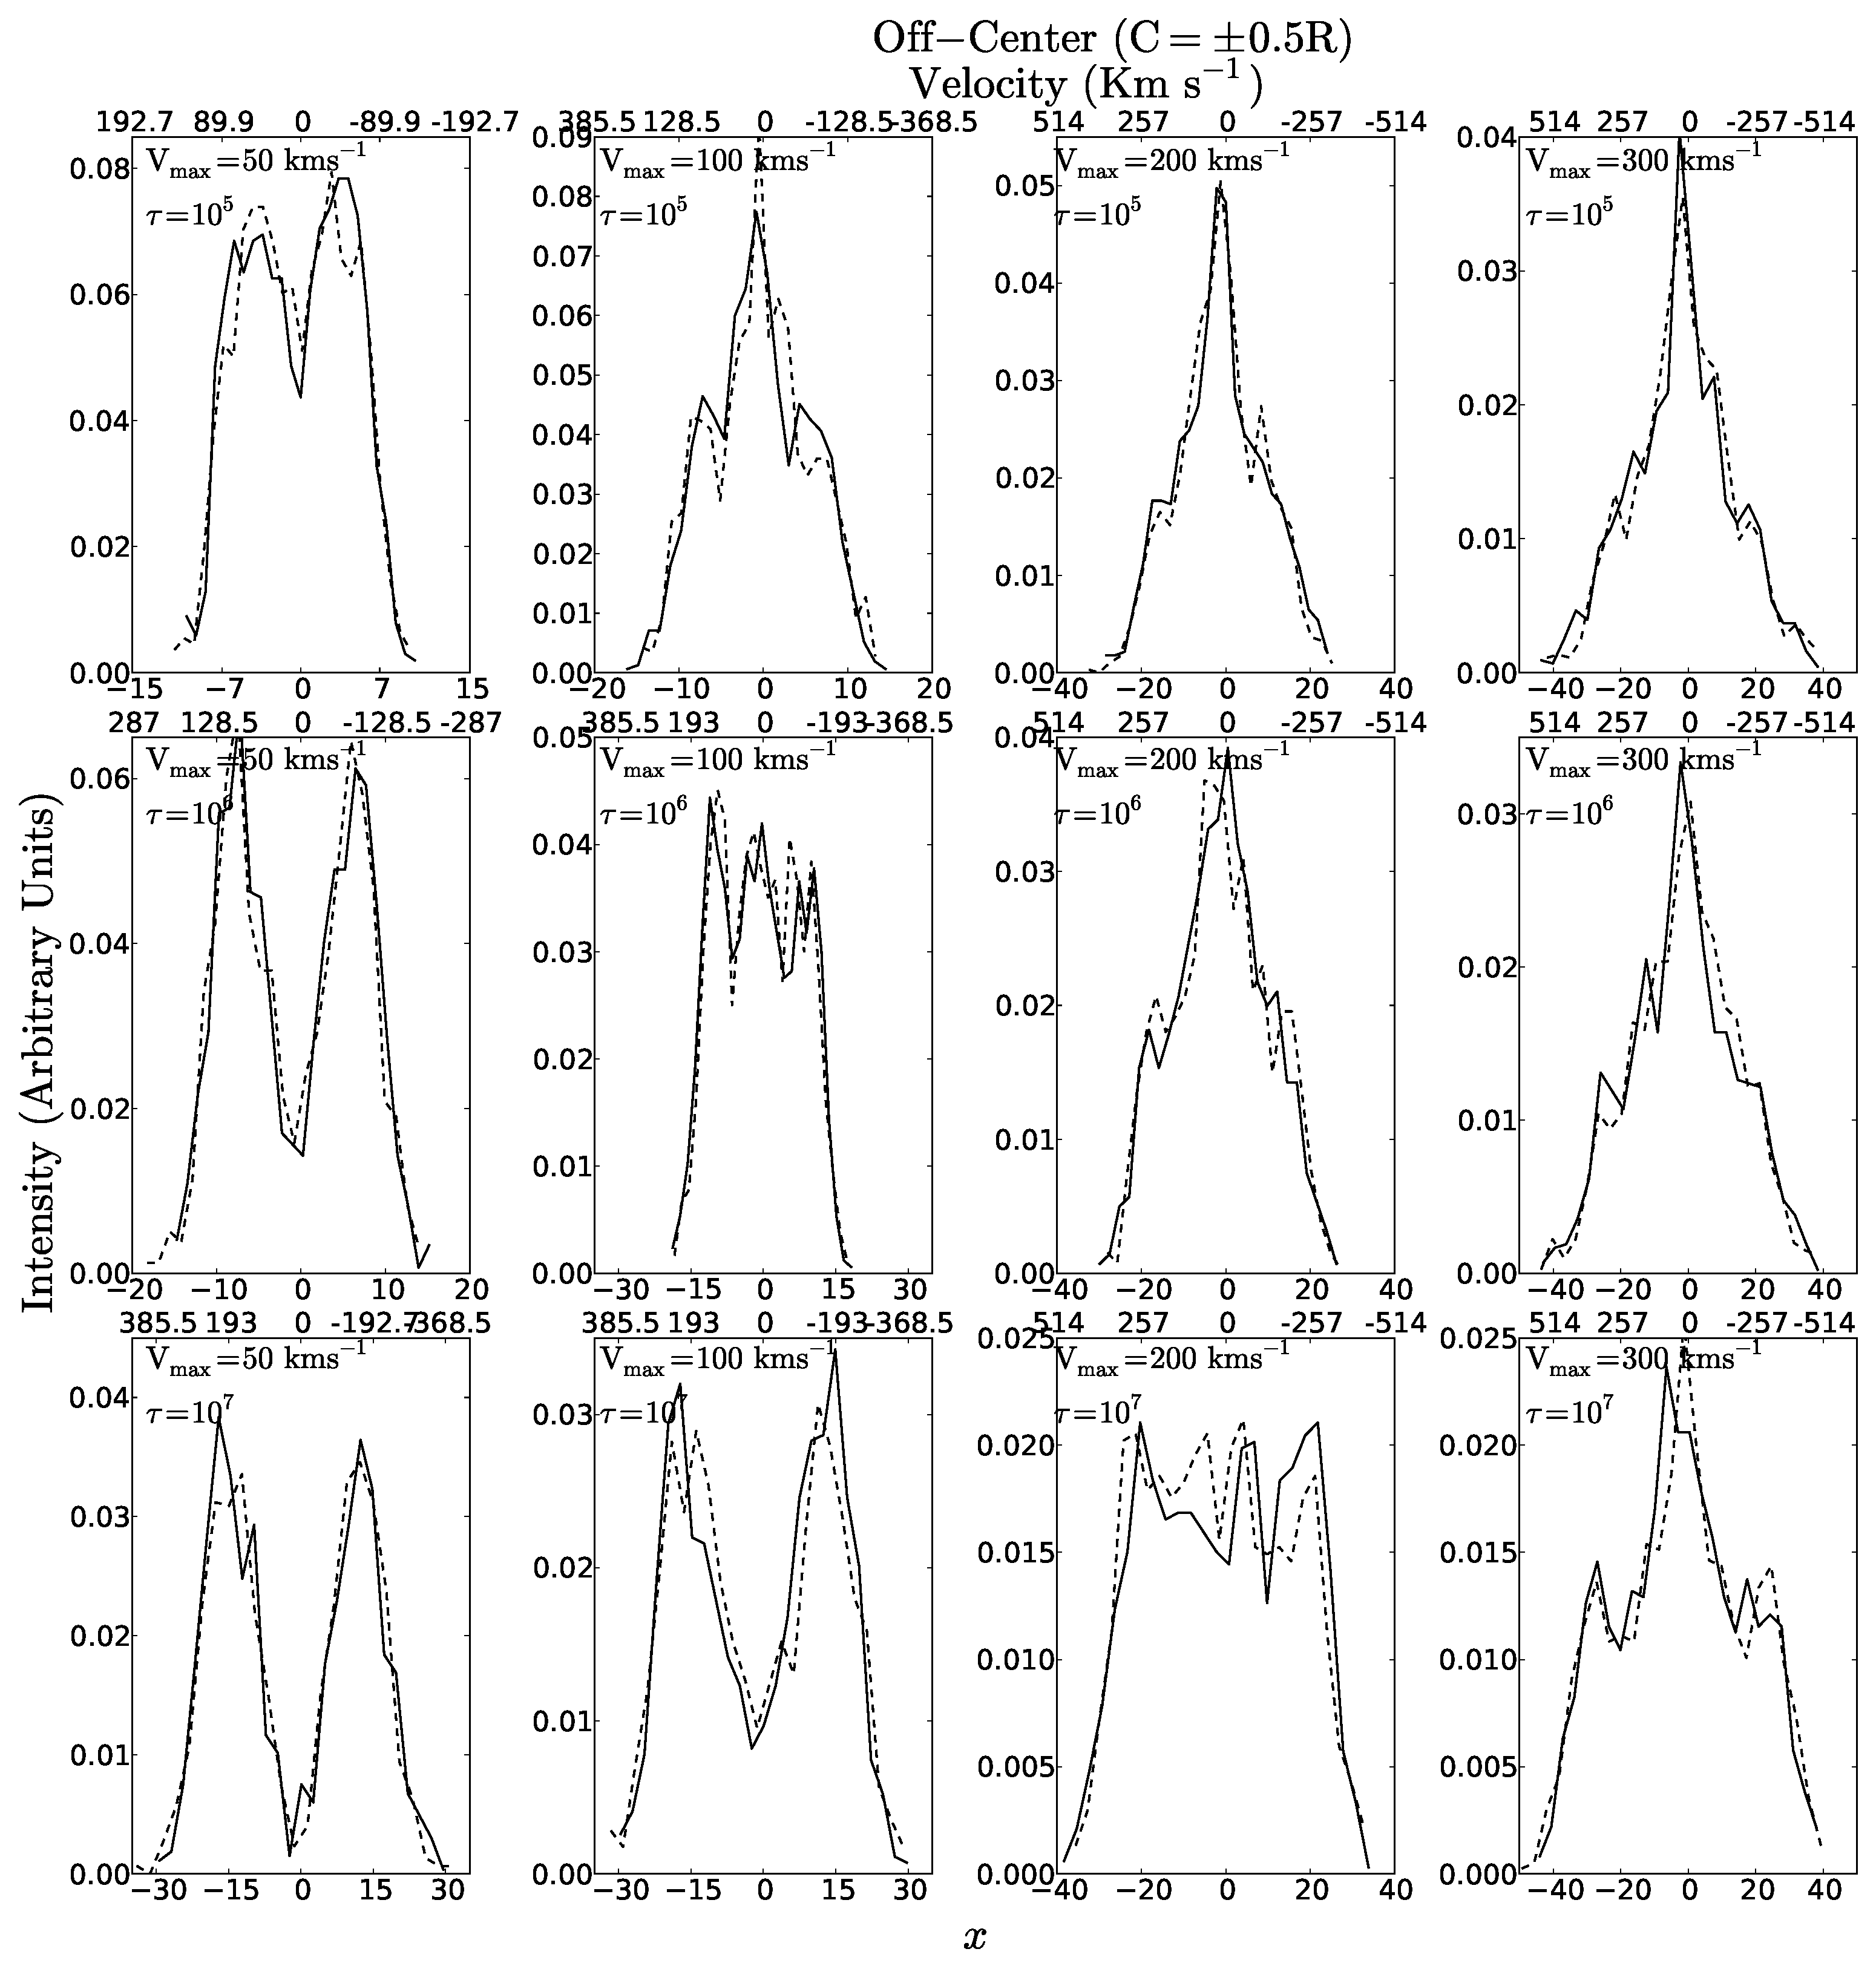
\includegraphics[scale=0.3]{f10.eps}
\end{center}
\caption{\ly profiles for the off-centered emission. Dashed/solid
  lines represents spheres centered at $-0,5R/+0.5R$ respectively.
   \label{fig:OC_profiles}} 
\end{figure*}

\subsection{Three-Peak Profiles}
\label{sec:3p}

\begin{figure*}
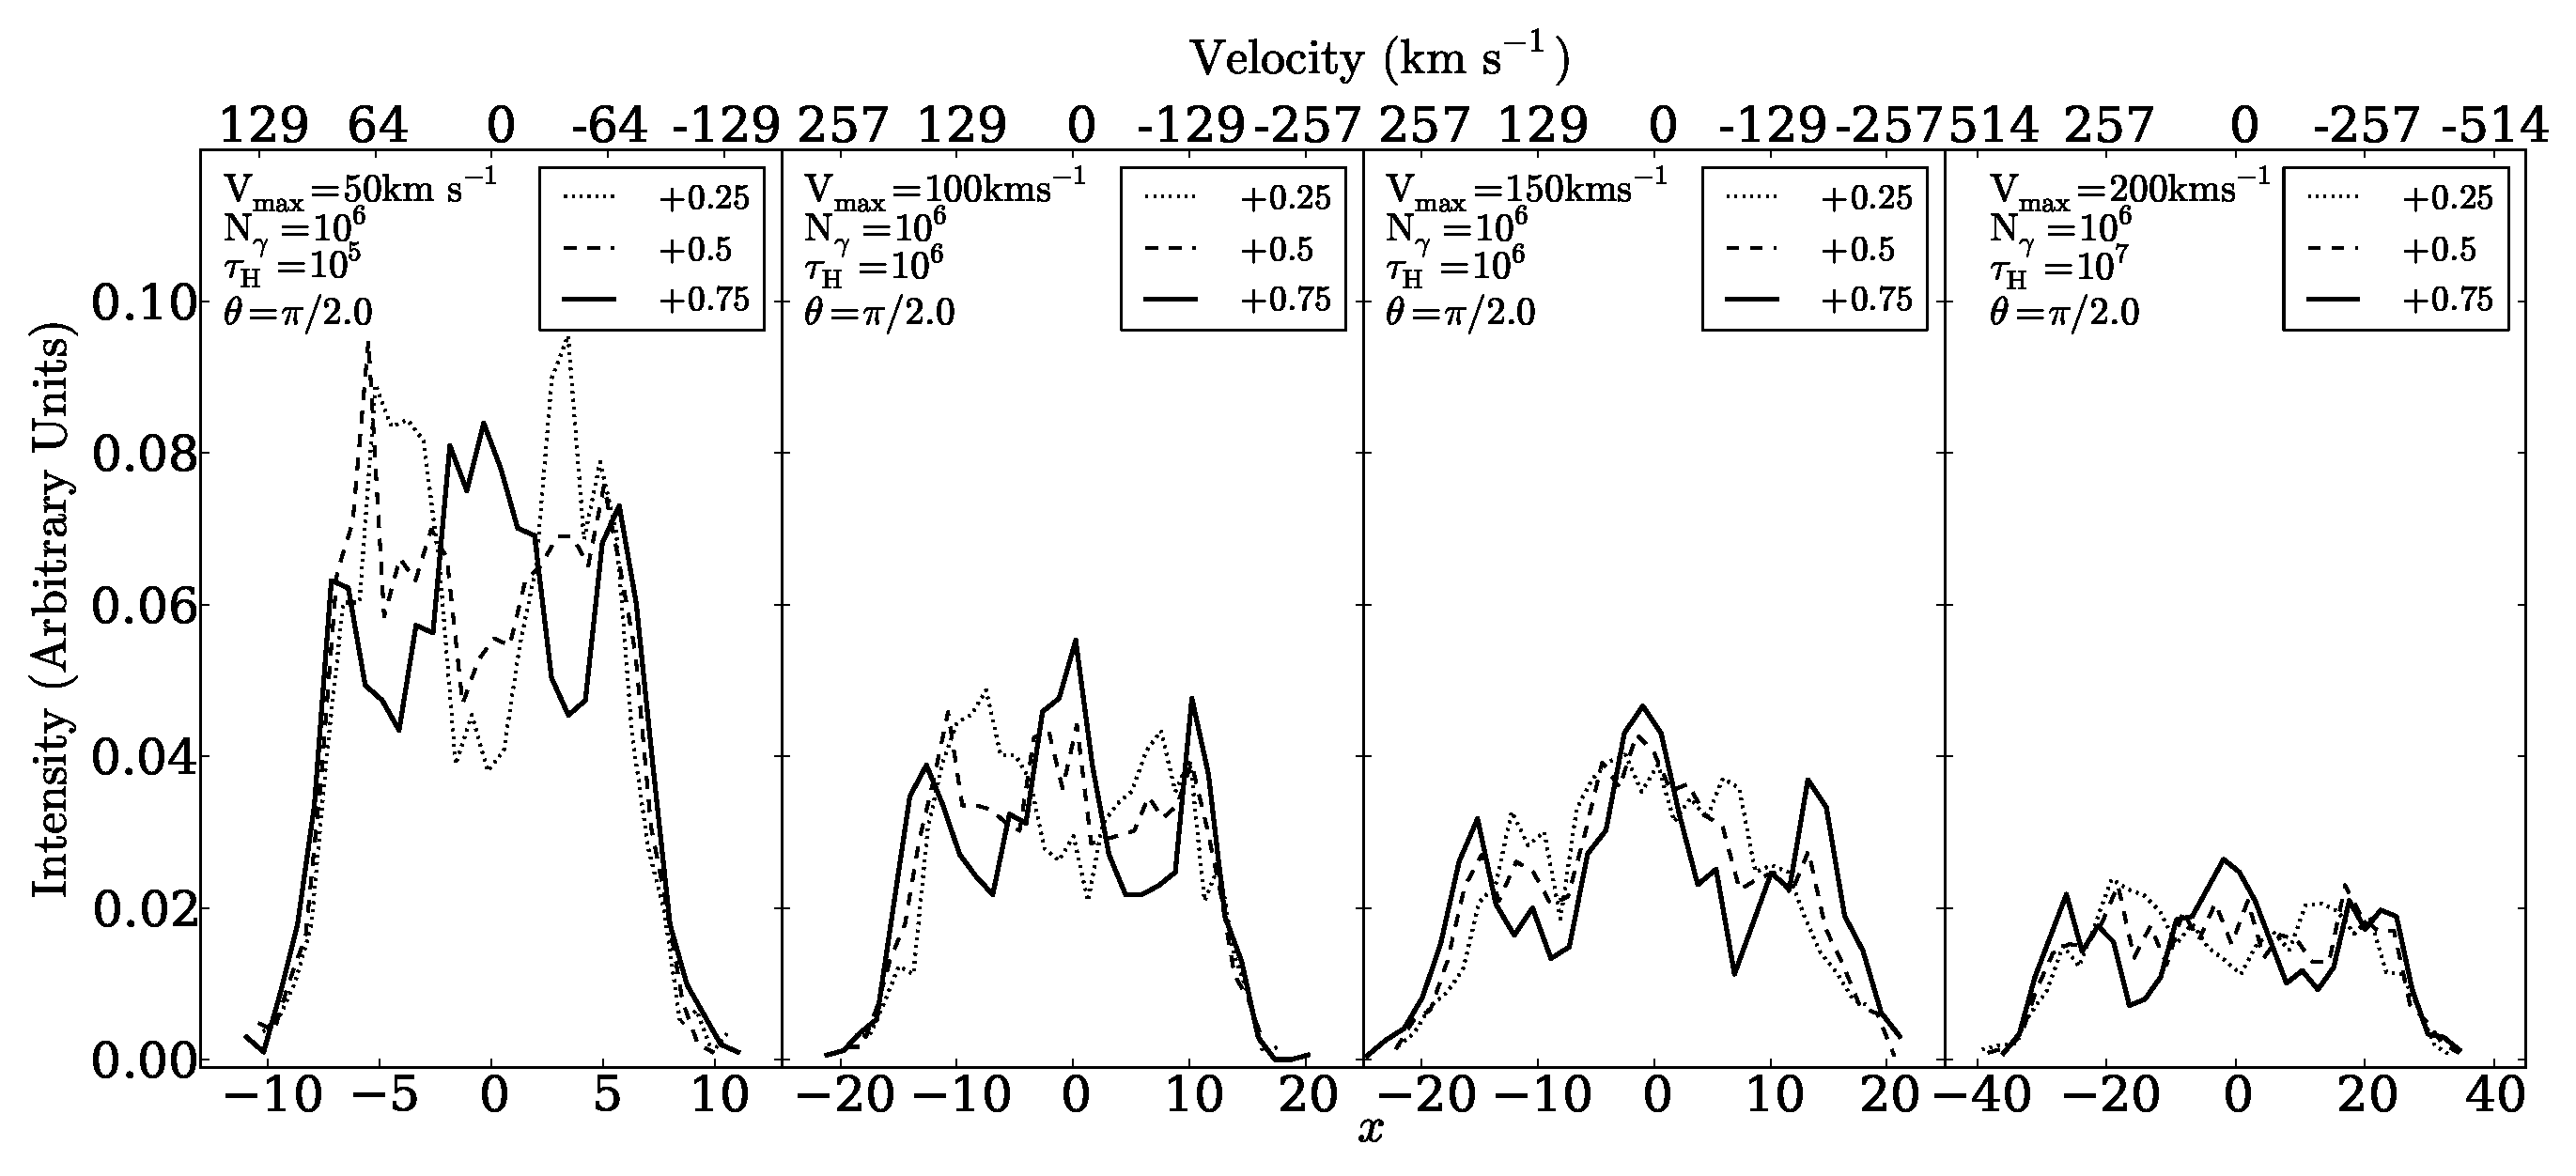
\includegraphics[scale=0.3]{f11.eps}
\caption{Triple peaked profiles for three different off-center positions
  $C=0.25R$ (doted line), $C=0.5R$ (dashed line) \& $C=0.75R$ (solid
  line) and for different rotational velocities.  
   \label{fig:3p_profiles}} 
\end{figure*}


Rotation breaks the spherical symmetry of the static model and
introduces the rotation axis as a preferred direction. This motivates
us to study the anisotropy of the outgoing photons. In order to study
possible deviations with respect to an isotropic flux we follow
\cite{Zheng2013} to estimate the flux as a function of the angle
$\Theta$ formed by the outgoing photons and the observer. Figure
\ref{fig:OCspheres} presents a geometric scheme to clarify the
definition of all relevant directions in the problem.

An estimator for the anysotropy is represented by
%
\begin{equation}
F(\mu) = \frac{2\Delta N}{N\Delta \mu}, 
\end{equation} 
%
where $\mu=\cos\Theta$, $N$ is the total number of outgoing photons,
$\Delta N$ is the number of photons in a angular bin $\Delta
\Theta$. This definition satisfies the condition
$\int_{-1}^{1}F(\mu)d\mu/2=1$.  With this definitions, the isotropic
emission is characterized by a flat $F(\mu)$ distribution. 


Figure \ref{fig:OCspheres} presents the results for the $F(\mu)$
distribution for an sphere with $\tau_{\rm H}=10^{7}$ and $V_{\rm
  max}=200$\kms. The dashed and dotted lines represent the homogeneous
and central source distribution, respectively. This shows that the
the  anisotropy induced by rotation is at the $3\%$ level. We
performed the same test with all the models and find that the
variation in $\mu$ does not depend on the rotational velocity;
however, high optical depth values can increase the variation of
$\mu$ up to a $15\%$. 

We also explore a different source of anisotropy by studying the effect
of radiation sources located in off-centered spheres with respect to
the gas distribution. Figure \ref{fig:OCspheres} shows the two
spherical regions we define to test for this effect. Each has a radius
of $0.5R$, where $R$ is the radius of the gaseus sphere. With an
observer located along the $\hat{j}$ direction, we pick two possible
positions to center the spheres along the $\hat{k}$ axis: $\pm C\hat{k}$. In
this configuration the emitting sphere centered on $+C\hat{k}$ moves
away from the observer and the sphere centered on $-C\hat{j}$ moves
towards the observer. 


In this case the $\mu$ distribution is not homogeneous as shown in
Figure \ref{fig:muhisto}. The off-center emision shows a variation at
the level of $20\%$ in intensity with the angle $\Theta$. {\bf Como se
ven los plots de otras velocidades y tau? Tambien son variaciones del
20\%?}. This variation implies that that the line is more intense in
the plane perpendicular to the rotation axis. 


We also explore the effects of off-centered emission in the line
morphology. Figure \ref{fig:OC_profiles} show sthe spectra for the two
off-centered emitting spheres located at $C=\pm0.5R$.  In this case we
only use photons that have outgoing directions aligned with the
observer i.e. $0.9 <\vert \mu \vert < 1.0$. We do not find any strong
asymmetry in the line morphology.  


However, we find some cases where there is a possible signature of
three peaks. This is only present in some models ($\tau = 10^6,
V=100$\kms and $\tau = 10^7, V=300$\kms) and could be the result of
two competing effects: the rise in the line's center as the photons in
the photosphere escape in a single excursion and the broadening in the
two peaks as the photons closer from the center have to scatter to
escape. 

%JEFR

As mentioned above Off-centered emission shows signs of three peak 
profiles, to analyse this in more detail we use the same method of the spheres
explained in \S \ref{sec:off-center}. We select spheres at $C=(\pm 0.25R, \pm0.5R, \pm0.75R)$ with a radii of
$0.25R$ for all the models, for those who present signs of three peak profiles such as 
$(V_{max}=50km$ $s^{-1}$ \& $\tau_{H}=10^{5}), (V_{max}=100km$ $s^{-1}$ \& $\tau_{H}=10^{6}), 
(V_{max}=200km$ $s^{-1}$ \& $\tau_{H}=10^{7})$ we made another run with $\tau_{\gamma}=10^{6}$ 
with the aim of get stronger profiles. 

Figure \ref{fig:3p_profiles} shows our findings, in order to get such profiles 
a relation between optical depth, rotational velocity and $C$ must be accomplish.
In particular we found that for the outer spheres $C=\pm 0.75$ the three
peak arises for all of our models with $\tau_{\gamma}=10^{6}$ this is due to 
the fact that the wings of the line move away from the central part as $C$ increase. 
Another requirement is that a high optical depth must be balanced with a high velocity 
in order to make the wings and the central peak similar in 
height, for models in which the velocity is low spheres at $C = \pm 0.25$ produce 
noise three peak profiles due to the high value of $\tau_{H, r}$.

Figure \ref{fig:3p_res} show that even with a low resolution a three-peak profile 
would be observed, this is important for observational porpoises due to the finite 
spectral resolution.

\begin{figure}
\begin{center}
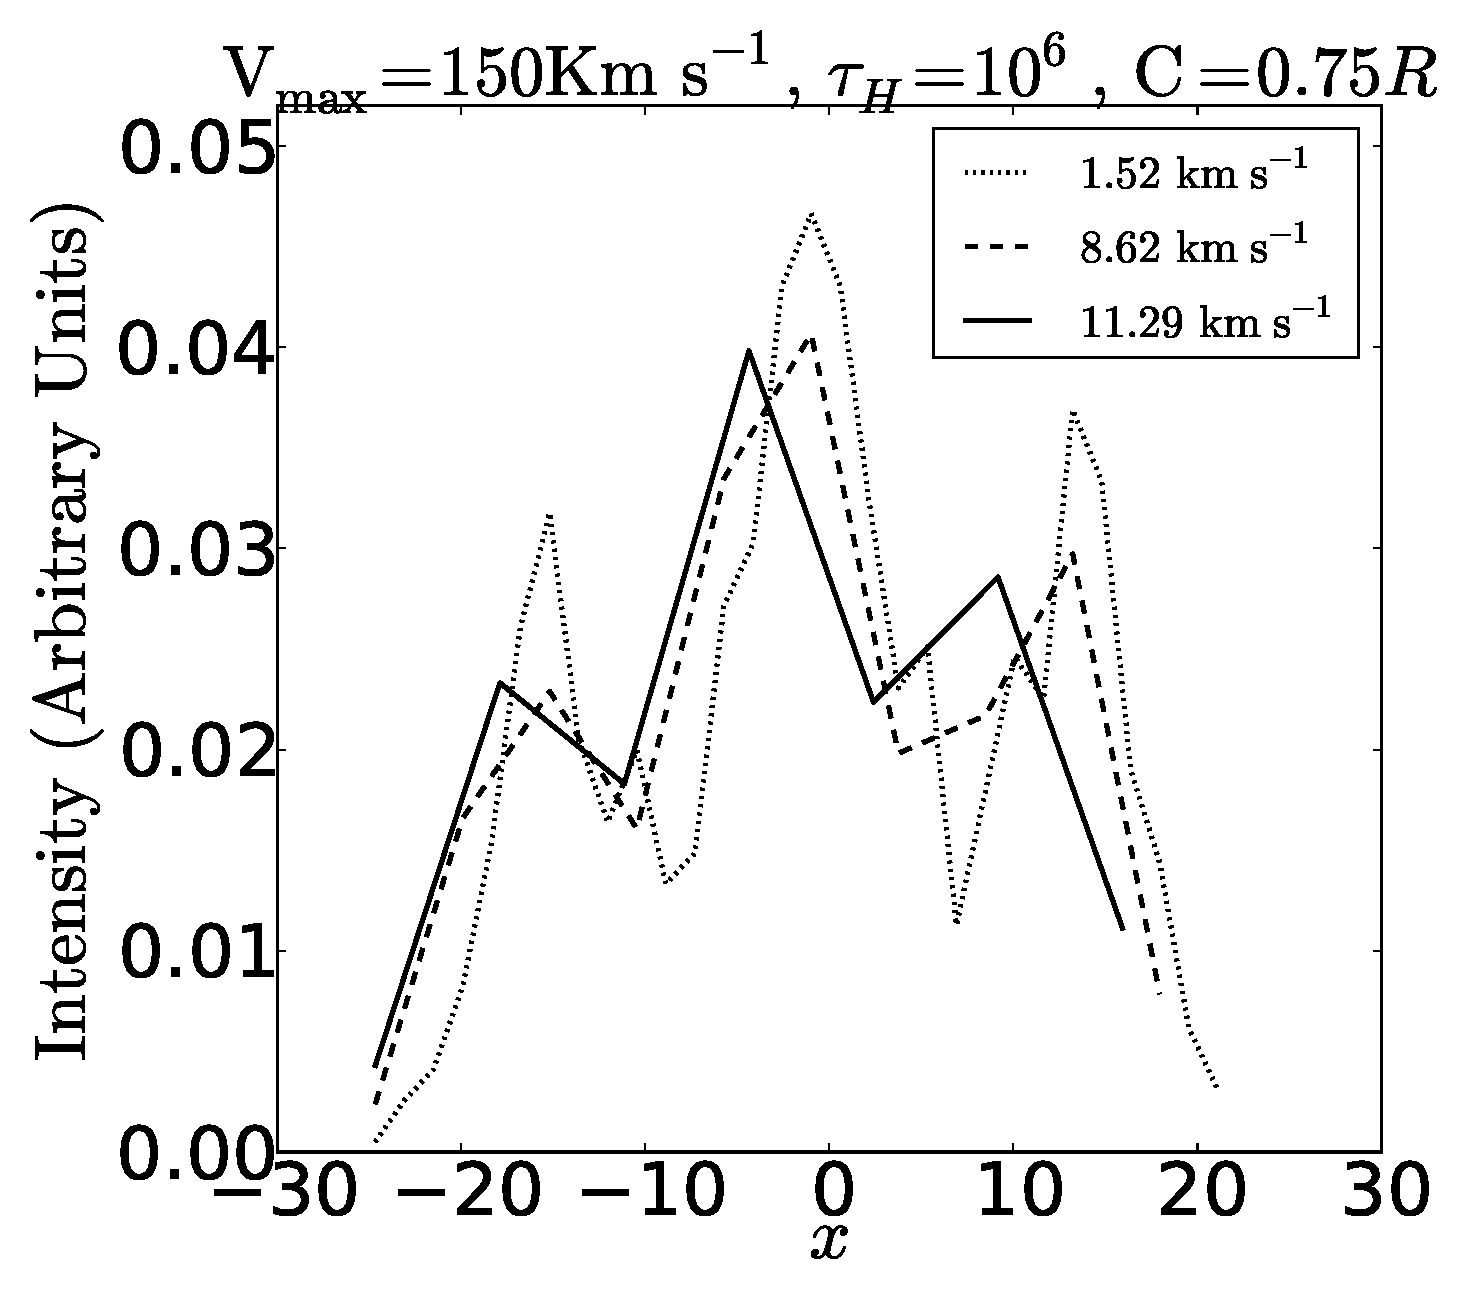
\includegraphics[scale=0.3]{f12.eps}
\end{center}
\caption{Three-Peak profiles for different resolutions:Low (Solid), medium(dashed), high(doted), 
   \label{fig:3p_res}} 
\end{figure}


\section{Discussion}
\label{sec:discussion}

Gas bulk rotation has a noticeable effect on the morphology of the
 \ly line. In this section we discuss the implications of these
 findings for the interpretation of available observational data. Our
 discussion focuses on the qualitative aspects of diverse
 morphological features observed by \cite{Kulas12} and \cite{Yamada2012}


We follow a classification of \ly profiles made by
\cite{Kulas12}. They presented observational results for star forming
galaxies at $z=2$-$3$ with multiple peaks in their \ly emission.
They classified the observed lines into five groups. In Group I the
red peak is stronger than the blue, while in Group II the blue peak is
stronger, in both cases the peaks are symmetrically located around the
line center. In Group III the blue peak also dominates but there is an
overall redward shift of the zero point. Group IV presents two similar
peaks symmetrically located around the zero point and Group V galaxies show
three peaks. 

The asymmetries in Groups I, II  and III cannot be explained by
rotation. However, some galaxies in those groups have a high flux between
the two peaks; an effect that can be induced by rotation. The same
argument applies to galaxies in the group IV in which the flux
in between of the two peaks is high ($ \geq 70 \%$ of the intensity in
the highest peak). Finally, the triple peaked lines in Galaxies in
Group V can be easily reproduced by rotation with off-centered
emission given the right amount of asymmetry between the emitting
region and neutral hydrogen distribution. 

Another relevant sample of observations was presented by \cite{Yamada2012} 
for 91 LAEs at $z=3.1$. They find that $\sim 33 \%$ of the galaxies present 
a single peak profile. Some of the peaks have a strong symmetry, while
others do not. The symmetric single peaked profile can be explained by
rotation effects, while the asymmetric cases naturally arise in
outflow/inflow models \citep{Verhamme2008, Dijkstra06}. Among the 91
LAEs, 8 reveal triple peaked profiles with a central peak and two
smaller peaks at the redder and bluer side, a feature that is present
in our off-center emission models with rotation Figure \ref{fig:3p_profiles}. 

The presence of single peaked profiles has been associated to
inflow/outflow dynamics \citep{XXX}. In this paper we show that gas
bulk rotation can also be considered as a probable origin for that
behavior, provided that the observed single peak is highly
symmetric. Similarly, in the case of double peaked lines with a high
level of flux at the line center, rotation also deserves to be considered in
the pool of possible bulk flows responsible for that feature,
specially if the two peaks have similar intensities. The case of
triple peaked lines is another clear feature of gas rotation under the
additional condition of an off-centered emission. 

\section{Conclusions}
\label{sec:conclusions}

This paper quantifies for the first time in the literature the effects
of rotation in the morphology of the \ly emission line in star forming
galaxies.  The results are based on the study of an homogeneous sphere
of gas with solid body rotation. We explore a range of models by varying
the rotational speed, hydrogen optical depth, dust optical depth and
initial distribution of \ly photons with respect to the gas
density. As a cross-validation, we obtain our results from two
independently developed Monte-Carlo radiative transfer codes. 

Our main result is that rotation clearly impacts the \ly line
morphology. Double peaked lines can make transitions into single
peaked lines as the rotational velocity increases. In the case of
off-centered emission result into triple peaked lines for certain
values of optical depth and rotational velocities. 

Quantitatively the main results of our study are summarized in the
following items. 

\begin{itemize}

\item The line width increases with rotational velocity. The line with
  approximately follows the functional form $W^2 = W_{
    0}^2 + (V_{\rm max}/\lambda)^2$ where $W_{0}$ indicates the line
  width for the static case. $\lambda$ is a constat determined from
  the radiative transfer results it is $\lambda_{\rm c}=XX$ and
  $\lambda_{\rm h}=YY$ for the central and homogeneous source
  distribution, respectively.


\item A single peaked line emerges for high rotational velocities in
  the case of homgeneously distributed sources. The cases of single
  peaked lines occur when the rotational velocity is larger than the
  line width measured in the static case.


\item For central sources we find that the number of scatterings
does not significantly decrease with rotation, this is due to the 
fact that the vast majority of scatterings events are resonant, 
during which the mean free path is very short and the effect of gas
bulk rotation is not enough to affect \ly photons.
The escape fraction does not depend on the rotational velocity neither
the position of the peaks, but there is an increase 
in the flux on the central parts of the line for high rotational 
velocities.

\item For homogeneous sources we find that the changes in the
line morphology are linked to the reduction in the average number of
scatterings. In the second part of \S \ref{sec:widthpeak} we show
that, as rotational velocity increases, a large fraction of photons
escape with less than $10$ scatterings and on average 
with $40\%$ less scatterings than in the static case. This makes highly improbable 
that a photon's frequency can move away from the line's center. 
In \S \ref{sec:widthpeak} For typical column densities of $N_{HI}=1e^{19}-1e^{20}$, 
we find that rotational velocities of 100-300 \kms broaden the line profile up 
to a factor of $2-3$ in comparison to the static case. Simultaneously, the
flux in the line center also increases with rotational velocity. This
increase induces the transition from a double peak to a single peak
line in the models where the radiation sources are homogeneously
distributed. Also the escape fraction increase by factors of $2-10$ with 
respect to the slab with centrally sources.

\item For non-symmetric sources we find that three peak profiles
could emerge for models in which the rotational velocity is the necessary 
to give rise to a central peak, but not that high to decrease the
amount of photons in the wings. When initial off-center sources are 
selected from the outer parts of the galaxy the wings of the line are stronger.
Also we do not find any considerable asymmetries in the line produced by off-center 
emission.
\end{itemize}

Comparing our results with recent observed LAEs we find that many 
morphological features such as high central line flux, single peak
profiles and multi-peaked profiles could be explained by gas bulk 
rotation present in these LAEs.


\section*{Acknowledgements}

JNGC acknowledges financial support from Universidad de los
Andes. 

JEFR acknowledges financial support from Vicerrectoria de
Investigaciones at Universidad de los Andes through a FAPA grant.

We thank the International Summer School on AstroComputing
2012 organized by the University of California High-Performance
AstroComputing Center (UC-HiPACC) for providing computational
resources where some of the calculations were done. 




\bibliographystyle{apj}
\bibliography{references} 


\end{document}


